\mfpicnumber{1}

\opengraphsfile{GraphsofSineandCosine}

\setcounter{footnote}{0}

\label{GraphsofSineandCosine}

On page \pageref{cosinesineequationsrealnumbers}, we discussed how to interpret the sine and cosine of real numbers.  To review, we identify a real number  $t$ with an oriented angle $\theta$ measuring $t$ radians\footnote{which, you'll recall  essentially `wraps the real number line around the Unit Circle}   and define $\sin(t) = \sin(\theta)$ and $\cos(t) = \cos(\theta)$.  Since every real number can be identified with one and only one angle $\theta$ this way, the domains of the functions $f(t) = \sin(t)$ and $g(t) = \cos(t)$ are all real numbers, $(-\infty, \infty)$.

\smallskip

When it comes to range, recall that the sine and cosine of angles are coordinates of points on the Unit Circle and hence, each  fall between $-1$ and $1$ inclusive.  Since the real number line,\footnote{in particular the interval $[0, 2\pi)$} when wrapped around the Unit Circle completely covers the circle, we can be assured that every point on the Unit Circle corresponds to at least one real number.  Putting these two facts together, we conclude the range of $f(t) = \sin(t)$ and $g(t) = \cos(t)$ are both $[-1,1]$.  We summarize these two important facts below.


\smallskip

\colorbox{ResultColor}{\bbm

\begin{thm} \label{cosinesinefunctiondomainrange}  \textbf{Domain and Range of the Cosine and Sine Functions:} 

\vspace{.2in}

\begin{tabular}{ll}

\hspace{.3in} $\bullet \, $ The function $f(t) = \sin(t)$ & \hspace{.8in} $\bullet \, $ The function $g(t) = \cos(t)$ \\ [4pt]
\hspace{.5in} -- has domain $(-\infty, \infty)$ & \hspace{1in} -- has domain $(-\infty, \infty)$ \\ [4pt]
\hspace{.5in} -- has range $[-1,1]$ & \hspace{1in} -- has range $[-1,1]$ \\ [4pt]

\end{tabular}

\end{thm}

\ebm}

\smallskip

Our aim in this section is to become familiar with the graphs of $f(t) = \sin(t)$ and $g(t) = \cos(t)$.  To that end, we begin by making a table and plotting points.  We'll start by graphing $f(t) = \sin(t)$ by making a table of values and plotting the corresponding points.  We'll keep the independent variable `$t$' for now and use the default `$y$' as our dependent variable.\footnote{Keep in mind that we're using `$y$' here to denote the \textit{output} from the sine function.  It is a coincidence that the $y$-values on the graph of $y=\sin(t)$ correspond to the $y$-values on the Unit Circle.}  Note in the graph below, on the right,  the scale of the horizontal and vertical axis is far from 1:1.  (We will present a more accurately scaled graph shortly.)


\hspace{.5in} \begin{tabular}{m{2.7in}m{3in}}
\setlength{\extrarowheight}{2pt}
\[ \begin{array}{|r||r|r|}  

\hline

 t & \sin(t) & (t,\sin(t)) \\ \hline
0  & 0 & (0, 0) \\ [2pt]   \hline
\frac{\pi}{4}  & \frac{\sqrt{2}}{2} & \left(\frac{\pi}{4}, \frac{\sqrt{2}}{2}\right) \\ [2pt] \hline 
\frac{\pi}{2}  & 1 & \left(\frac{\pi}{2}, 1\right) \\ [2pt] \hline 
\frac{3\pi}{4}  & \frac{\sqrt{2}}{2} & \left(\frac{3\pi}{4}, \frac{\sqrt{2}}{2}\right) \\ [2pt] \hline 
\pi & 0 & (\pi, 0) \\ [2pt] \hline 
\frac{5\pi}{4}  & -\frac{\sqrt{2}}{2} & \left(\frac{5\pi}{4}, -\frac{\sqrt{2}}{2}\right) \\ [2pt] \hline 
\frac{3\pi}{2}  & -1 & \left(\frac{3\pi}{2}, -1 \right) \\ [2pt] \hline 
\frac{7\pi}{4}  & -\frac{\sqrt{2}}{2} & \left(\frac{7\pi}{4}, -\frac{\sqrt{2}}{2}\right) \\ [2pt] \hline 
2\pi  & 0 & (2\pi, 0) \\  [2pt] \hline
\end{array} \] \setlength{\extrarowheight}{0pt} &

\begin{mfpic}[25][50]{-1}{7}{-1.5}{1.5}
\point[4pt]{(0,0), (0.7854,0.7071), (1.5708,1), (2.3562,0.7071), (3.1416, 0), (3.9270,-0.7071), (4.7124,-1), (5.4978,-0.7071), (6.2832,0)}
\axes
\tlabel[cc](7,-0.15){\scriptsize $t$}
\tlabel[cc](0.25,1.5){\scriptsize $y$}
\tcaption{Graphing $y = \sin(t)$.}
\xmarks{0.7854, 1.5708, 2.3562, 3.1416, 3.9270, 4.7124,5.4978,6.2832 }
\ymarks{-1,1}
\tlpointsep{4pt}
\scriptsize
\axislabels {x}{{$\frac{\pi}{4}$} 0.7854, {$\frac{\pi}{2}$} 1.5708, {$\frac{3\pi}{4}$} 2.3562, {$\pi$} 3.1416, {$\frac{5\pi}{4}$} 3.9270, {$\frac{3\pi}{2}$} 4.7124, {$\frac{7\pi}{4}$} 5.4978, {$2\pi$} 6.2832}
\normalsize
\axislabels {y}{{\scriptsize $-1$} -1, {\scriptsize $1$} 1}
\penwd{1.1pt}
\function{0, 6.2832, 0.1}{sin(x)}
\end{mfpic} \\

\end{tabular}

If we plot additional points, we soon find that the graph repeats itself.   This shouldn't come as too much of a surprise considering Theorem \ref{coterminalsamcosinesinethm}.  In fact, in light of that theorem, we expect the function to repeat itself every $2\pi$ units.  Below is a more accurately scaled graph highlighting the portion we had already graphed above.  The graph is often described as having a `wavelike' nature and is sometimes called a \index{wave ! sine}\index{sine wave} \textbf{sine wave} or, more technically, a \index{sinusoid}\textbf{sinusoid}.

\smallskip

\begin{center}

\begin{mfpic}[15]{-13}{13}{-1.5}{1.5}
\axes
\point[4pt]{(0,0), (6.2832,0)}
\tlabel[cc](13,-0.5){\scriptsize $t$}
%\tlabel[cc](0.5,1.5){\scriptsize $y$}
\tlabel[cc](0.5,1.25){\scriptsize $1$}
\tlabel[cc](0.5,-1){\scriptsize $-1$}
\tcaption{A more accurately scaled graph of $f(t) = \sin(t)$.}
\ymarks{-1,1}
\arrow \reverse \arrow \function{-12, 12, 0.1}{sin(x)}
\penwd{1.5pt}
\function{0, 6.2832, 0.1}{sin(x)}
\end{mfpic}

\end{center}

Note that by copying  the highlighted portion of the graph and pasting it end-to-end, we obtain the entire graph of $f(t) = \sin(t)$.  We give this `repeating' property a name.

\smallskip

\colorbox{ResultColor}{\bbm

\begin{defn} \label{periodic} \textbf{Periodic Functions:} A function $f$ is said to be \textbf{periodic}\index{function ! periodic}\index{periodic function}  if there is a real number $c$ so that $f(t+c) = f(t)$ for all real numbers $t$ in the domain of $f$.  The smallest positive number $p$ for which $f(t+p) = f(t)$ for all real numbers $t$ in the domain of $f$, if it exists, is called the \textbf{period} of $f$. \index{period ! of a function}

\end{defn}

\ebm}

\medskip

We have already seen a family of periodic functions in Section \ref{ConstantandLinearFunctions}:  the constant functions.  However, despite being periodic a constant function has no period.  (We'll leave that odd gem as an exercise for you.)  

\smallskip

Returning to $f(t) = \sin(t)$, we see that by Definition \ref{periodic}, $f$ is periodic since $\sin(t + 2\pi) = \sin(t)$.  To determine the period of $f$, we need to find the smallest real number $p$ so that $f(t+p) = f(t)$ for all real numbers $t$ or, said differently, the smallest positive real number $p$ such that $\sin(t+p) = \sin(t)$  for all real numbers $t$.  

\smallskip

We know that $\sin(t + 2\pi) = \sin(t)$ for all real numbers $t$ but the question remains if any smaller real number will do the trick.  Suppose $p>0$ and $\sin(t + p) = \sin(t)$ for all real numbers $t$.  Then, in particular, $\sin(0+p) = \sin(0)=0$ so that $\sin(p) = 0$.  From this we know $p$ is a multiple of $\pi$.  Since $\sin\left(\frac{\pi}{2} \right)  \neq \sin\left(\frac{\pi}{2} + \pi \right) $, we know $p \neq \pi$.  Hence, $p  = 2\pi$ so the period of $f(t) = \sin(t)$ is $2\pi$. 

\smallskip

Having period $2\pi$ essentially means that we can completely understand everything about the function  $f(t) =  \sin(t)$ by studying \textit{one} interval of length $2\pi$, say $[0,2\pi]$.\footnote{Technically, we should study the interval $[0,2\pi)$,\footnotemark since whatever happens at $t=2\pi$ is the same as what happens at $t=0$.  As we will see shortly, $t=2\pi$ gives us an extra `check' when we go to graph these functions.} \footnotetext{In some advanced texts, the interval of choice is $[-\pi, \pi)$.}  For this reason, when graphing sine (and cosine) functions, we typically restrict our attention to graphing these functions over the course of one period to produce one \index{cycle ! of $\sin(t)$ and $\cos(t)$}\textbf{cycle} of the graph. 
 
\smallskip


Not surprisingly, the graph of $g(t) = \cos(t)$ exhibits similar behavior as $f(t) = \sin(t)$ as seen below.\footnote{Here note that the dependent variable `$y$' represents the outputs from  $g(t) = \cos(t)$ which are $x$-coordinates on the Unit CIrcle.}  

\hspace{.5in} \begin{tabular}{m{2.7in}m{3in}}
\setlength{\extrarowheight}{2pt}
\[ \begin{array}{|r||r|r|}  

\hline

 t & \cos(t) & (t,\cos(t)) \\ \hline
0  & 1 & (0, 1) \\ [2pt]   \hline
\frac{\pi}{4}  & \frac{\sqrt{2}}{2} & \left(\frac{\pi}{4}, \frac{\sqrt{2}}{2}\right) \\ [2pt] \hline 
\frac{\pi}{2}  & 0 & \left(\frac{\pi}{2}, 0\right) \\ [2pt] \hline 
\frac{3\pi}{4}  & -\frac{\sqrt{2}}{2} & \left(\frac{3\pi}{4}, -\frac{\sqrt{2}}{2}\right) \\ [2pt] \hline 
\pi & -1 & (\pi, -1) \\ [2pt] \hline 
\frac{5\pi}{4}  & -\frac{\sqrt{2}}{2} & \left(\frac{5\pi}{4}, -\frac{\sqrt{2}}{2}\right) \\ [2pt] \hline 
\frac{3\pi}{2}  & 0 & \left(\frac{3\pi}{2}, 0 \right) \\ [2pt] \hline 
\frac{7\pi}{4}  & \frac{\sqrt{2}}{2} & \left(\frac{7\pi}{4}, \frac{\sqrt{2}}{2}\right) \\ [2pt] \hline 
2\pi  & 1 & (2\pi, 1) \\  [2pt] \hline
\end{array} \] \setlength{\extrarowheight}{0pt} &

\begin{mfpic}[25][50]{-1}{7}{-1.5}{1.5}
\point[4pt]{(0,1), (0.7854,0.7071), (1.5708,0), (2.3562,-0.7071), (3.1416, -1), (3.9270,-0.7071), (4.7124,0), (5.4978,0.7071), (6.2832,1)}
\axes
\tlabel[cc](7,-0.15){\scriptsize $t$}
\tlabel[cc](0.25,1.5){\scriptsize $y$}
\tcaption{Graphing $y = \cos(t)$.}
\xmarks{0.7854, 1.5708, 2.3562, 3.1416, 3.9270, 4.7124,5.4978,6.2832 }
\ymarks{-1,1}
\tlpointsep{4pt}
\scriptsize
\axislabels {x}{{$\frac{\pi}{4}$} 0.7854, {$\frac{\pi}{2}$} 1.5708, {$\frac{3\pi}{4}$} 2.3562, {$\pi$} 3.1416, {$\frac{5\pi}{4}$} 3.9270, {$\frac{3\pi}{2}$} 4.7124, {$\frac{7\pi}{4}$} 5.4978, {$2\pi$} 6.2832}
\normalsize
\axislabels {y}{{\scriptsize $-1$} -1, {\scriptsize $1$} 1}
\penwd{1.25pt}
\function{0, 6.2832, 0.1}{cos(x)}
\end{mfpic} \\

\end{tabular}

\smallskip

Like $f(t)=\sin(t)$, $g(t) = \cos(t)$ is a wavelike curve with period $2\pi$.   Moreover, the graphs of the sine and cosine functions have the same shape -  differing only in what appears to be a horizontal shift.  As we'll prove in Section \ref{MoreTrigonometricIdentities}, $\sin\left(t + \frac{\pi}{2}\right) = \cos(t)$, which means we can obtain the graph of $y=\cos(t)$ by shifting the graph of $y=\sin(t)$ to the left $\frac{\pi}{2}$ units.\footnote{Hence, we can obtain the graph of $y = \sin(t)$ by shifting the graph of $y = \cos(t)$ to the \textit{right} $\frac{\pi}{2}$ units: $\cos\left(t - \frac{\pi}{2} \right) = \sin(t)$.}


\smallskip

\begin{center}

\begin{mfpic}[15]{-13}{13}{-1.5}{1.5}
\axes
\point[4pt]{(0,1), (6.2832,1)}
\tlabel[cc](13,-0.5){\scriptsize $t$}
%\tlabel[cc](0.5,1.5){\scriptsize $y$}
\tcaption{The graph of $g(t) = \cos(t)$.}
\ymarks{-1,1}
\tlabel[cc](0.5,1.25){\scriptsize $1$}
\tlabel[cc](0.5,-1){\scriptsize $-1$}
\arrow \reverse \arrow \function{-12.5664, 12.5664, 0.1}{cos(x)}
\penwd{1.5pt}
\function{0, 6.2832, 0.1}{cos(x)}
\end{mfpic}

\end{center}

\smallskip

While arguably the most important property shared by  $f(t) = \sin(t)$ and $g(t) = \cos(t)$ is their periodic `wavelike' nature,\footnote{this is the reason they are so useful in the Sciences and Engineering} their graphs suggest these functions are both continuous and smooth.  Recall from Section \ref{GraphsofPolynomials} that, like polynomial functions, the graphs of the sine and cosine functions have no jumps, gaps, holes in the graph,  vertical asymptotes, corners or cusps.  

\smallskip

Note the graphs of both $f(t) = \sin(t)$ and $g(t) = \cos(t)$ meander  as $t \rightarrow -\infty$ or as $ \rightarrow \infty$.  Said differently, none of the limits  $\ds{\lim_{t \rightarrow -\infty} \sin(t)}$,   $\ds{\lim_{t \rightarrow \infty} \sin(t)}$, $\ds{\lim_{t \rightarrow -\infty} \cos(t)}$, or $\ds{\lim_{t \rightarrow \infty} \cos(t)}$ exist.  Even though these functions are `trapped' (or \index{bounded}\textbf{bounded}) between $-1$ and $1$, neither graph has any horizontal asymptotes.

\smallskip

Lastly, the graphs of  $f(t) = \sin(t)$ and $g(t) = \cos(t)$ suggest each enjoy one of the symmetries introduced in Section \ref{GraphsofPolynomials}.  The graph of $y = \sin(t)$ appears to be symmetric about the origin while the graph of $y = \cos(t)$ appears to be symmetric about the $y$-axis.  Indeed, as we'll prove in Section \ref{MoreTrigonometricIdentities}, $f(t) = \sin(t)$ is, in fact, an odd function: \footnote{The reader may wish to review Definitions  \ref{evenfunctiondefn} and  \ref{oddfunctiondefn} as needed.}  that is, $\sin(-t) = -\sin(t)$ and  $g(t) = \cos(t)$ is an even function, so $\cos(-t) = \cos(t)$.  

\smallskip

 We summarize all of these properties in the following result.

\smallskip

\colorbox{ResultColor}{\bbm

\begin{thm} \label{cosinesinefunctionprops}  \textbf{Properties of the Cosine and Sine Functions} \index{cosine ! properties of} \index{sine ! properties of}

\vspace{.2in}

\begin{tabular}{ll}

\hspace{.3in} $\bullet \, $ The function $f(t) = \sin(t)$ & \hspace{.8in} $\bullet \, $ The function $g(t) = \cos(t)$ \\
  & \\

\hspace{.5in} -- has domain $(-\infty, \infty)$ & \hspace{1in} -- has domain $(-\infty, \infty)$ \\ [4pt]
\hspace{.5in} -- has range $[-1,1]$ & \hspace{1in} -- has range $[-1,1]$ \\ [4pt]
\hspace{.5in} -- is continuous and smooth & \hspace{1in} -- is continuous and smooth \\ [4pt]
\hspace{.5in} -- is odd & \hspace{1in} -- is  even \\ [4pt]
\hspace{.5in} -- has period $2\pi$ & \hspace{1in} -- has period $2\pi$ \\ 

\end{tabular}

\smallskip

\hspace{.3in} $\bullet \, $ Conversion formulas:  $\sin\left(t + \frac{\pi}{2}\right) = \cos(t)$ and   $\cos\left(t - \frac{\pi}{2} \right) = \sin(t)$

\smallskip

\end{thm}

\ebm}

\smallskip

Now that we know the basic shapes of the graphs of $y = \sin(t)$ and $y = \cos(t)$, we can use the results of Section \ref{Transformations} to graph more complicated functions using transformations.  The fact that both of these functions are periodic means we only have to know what happens over the course of one period of the function in order to determine what happens to all points on the graph.  To that end, we graph the \index{fundamental cycle ! of $\sin(t)$ and $\cos(t)$}`\textbf{fundamental cycle}'  - the portion of each graph generated over the interval $[0, 2\pi]$ - for each  sine and cosine:

\begin{multicols}{2}

\begin{mfpic}[25][50]{-1}{7}{-1.5}{1.5}
\point[4pt]{(0,0), (1.5708,1), (3.1416, 0), (4.7124,-1), (6.2832,0)}
\axes
\tlabel[cc](7,-0.15){\scriptsize $t$}
\tlabel[cc](0.25,1.5){\scriptsize $y$}
\tlabel[cc](-0.5, -0.15){\scriptsize $(0,0)$}
\tlabel[cc](1.5708, 1.25){\scriptsize $\left(\frac{\pi}{2},1 \right)$}
\tlabel[cc](3.5, 0.15){\scriptsize $(\pi,0)$}
\tlabel[cc](4.7124, -1.25){\scriptsize $\left(\frac{3\pi}{2}, -1 \right)$}
\tlabel[cc](6.2832, 0.15){\scriptsize $(2 \pi,0)$}
\tcaption{The `fundamental cycle' of  $y = \sin(t)$.}
\xmarks{1.5708, 3.1416, 4.7124, 6.2832 }
\ymarks{-1,1}
\tlpointsep{4pt}
\scriptsize
\axislabels {x}{{$\frac{\pi}{2}$} 1.5708, {$\pi$} 3.1416, {$\frac{3\pi}{2}$} 4.7124,  {$2\pi$} 6.2832}
\normalsize
\axislabels {y}{{\scriptsize $-1$} -1, {\scriptsize $1$} 1}
\penwd{1.1pt}
\function{0, 6.2832, 0.1}{sin(x)}
\end{mfpic} 



\begin{mfpic}[25][50]{-1}{7}{-1.5}{1.5}
\point[4pt]{(0,1), (1.5708,0), (3.1416, -1), (4.7124,0), (6.2832,1)}
\axes
\tlabel[cc](7,-0.15){\scriptsize $t$}
\tlabel[cc](0.25,1.5){\scriptsize $y$}
\tlabel[cc](-0.5, 1){\scriptsize $(0,1)$}
\tlabel[cc](2, 0.15){\scriptsize $\left(\frac{\pi}{2},0 \right)$}
\tlabel[cc](3.1416, -1.25){\scriptsize $(\pi,-1)$}
\tlabel[cc](5.5, 0.15){\scriptsize $\left(\frac{3\pi}{2}, 0 \right)$}
\tlabel[cc](6.2832, 1.25){\scriptsize $(2 \pi,1)$}
\tcaption{The `fundamental cycle' of  $y = \cos(t)$.}
\xmarks{1.5708, 3.1416, 4.7124, 6.2832 }
\ymarks{-1,1}
\tlpointsep{4pt}
\scriptsize
\axislabels {x}{ {$\frac{\pi}{2}$} 1.5708, {$\pi$} 3.1416, {$\frac{3\pi}{2}$} 4.7124,  {$2\pi$} 6.2832}
\normalsize
\axislabels {y}{{\scriptsize $-1$} -1}
\penwd{1.1pt}
\function{0, 6.2832, 0.1}{cos(x)}
\end{mfpic}

\end{multicols}


In working through Section \ref{Transformations} , it was very helpful to track `key points' through  the transformations.  The `key points' we've indicated on the graphs above correspond to the quadrantal angles and generate the zeros and the extrema of functions. Since the quadrantal angles divide the interval $[0,2\pi]$ into four equal pieces, we shall refer to these angles henceforth  as the  `quarter marks.'    

\smallskip

It is worth noting that because the transformations discussed in Section \ref{Transformations} are linear,\footnote{See the remarks at the beginning of Section \ref{Transformations}.}  the \textit{relative spacing} of the points before and after the transformations remains the same.\footnote{If we use a linear function $f(t) = mt + b$ to transform the inputs, $t$, then  $\Delta[f(t)] = m \Delta t$.  That is, the change \textit{after} the the transformation, $m \Delta t$, is just a multiple of the change \textit{before} the transformation, $\Delta t$.}  In particular, wherever the interval $[0, 2\pi]$ is mapped, the quarter marks of the new interval correspond to the quarter marks of $[0, 2\pi]$.  (Can you see why?) We will exploit this fact in the following example.


\begin{ex}  \label{cosinesinegraphex1} Graph one cycle of the following functions. State the period of each.

\begin{multicols}{2}

\begin{enumerate}

\item  $f(t) = 3 \sin(2t)$

\item  $g(t) = 2 \cos\left(t +\frac{\pi}{2} \right) +1$

\end{enumerate}

\end{multicols}

{\bf Solution.}

\begin{enumerate}

\item One way to proceed is to use Theorem \ref{transformationsthm} and follow the procedure outlined there.   Starting with the fundamental cycle of $y= \sin(t)$, we divide each $t$-coordinate by $2$ and multiply each $y$-coordinate by 3 to obtain one cycle of $y = 3 \sin(2t)$.  

\begin{multicols}{2}

\begin{mfpic}[20]{-1}{7}{-3.5}{3.5}
\point[4pt]{(0,0), (1.5708,1), (3.1416, 0), (4.7124,-1), (6.2832,0)}
\axes
\tlabel[cc](7,-0.15){\scriptsize $t$}
\tlabel[cc](0.25,3.5){\scriptsize $y$}
\tlabel[cc](-0.5, -0.4){\scriptsize $(0,0)$}
\tlabel[cc](1.5708, 1.5){\scriptsize $\left(\frac{\pi}{2},1 \right)$}
\tlabel[cc](3.5, 0.4){\scriptsize $(\pi,0)$}
\tlabel[cc](4.7124, -1.5){\scriptsize $\left(\frac{3\pi}{2}, -1 \right)$}
\tlabel[cc](6.2832, 0.4){\scriptsize $(2 \pi,0)$}
\tcaption{The `fundamental cycle' of  $y = \sin(t)$.}
\xmarks{0.7854, 1.5708, 2.3562, 3.1416, 3.9270, 4.7124,5.4978,6.2832 }
\ymarks{-1,1}
\tlpointsep{4pt}
\scriptsize
\axislabels {x}{{$\frac{\pi}{4}$} 0.7854, {$\frac{\pi}{2}$} 1.5708, {$\frac{3\pi}{4}$} 2.3562, {$\pi$} 3.1416, {$\frac{5\pi}{4}$} 3.9270, {$\frac{3\pi}{2}$} 4.7124, {$\frac{7\pi}{4}$} 5.4978, {$2\pi$} 6.2832}
\normalsize
\axislabels {y}{{\scriptsize $-1$} -1, {\scriptsize $1$} 1, {\scriptsize $2$} 2, {\scriptsize $3$} 3, {\scriptsize $-2$} -2, , {\scriptsize $-3$} -3}
\penwd{1.1pt}
\function{0, 6.2832, 0.1}{sin(x)}
\end{mfpic} 


\begin{mfpic}[20]{-1}{7}{-3.5}{3.5}
\point[4pt]{(0,0), (0.7854,3), (1.5708, 0), (2.3562,-3), (3.1416,0)}
\axes
\tlabel[cc](7,-0.15){\scriptsize $t$}
\tlabel[cc](0.25,3.5){\scriptsize $y$}
\tlabel[cc](-0.5, 0.4){\scriptsize $(0,0)$}
\tlabel[cc](1.5, 3){\scriptsize $\left(\frac{\pi}{4},3 \right)$}
\tlabel[cc](0.9, -0.4){\scriptsize $\left( \frac{\pi}{2}, 0 \right)$}
\tlabel[cc](2.3562, -3.5){\scriptsize $\left(\frac{3\pi}{4}, -3 \right)$}
\tlabel[cc](3.1416, 0.4){\scriptsize $(\pi,0)$}
\tcaption{One cycle of $y = 3 \sin(2t)$.}
\xmarks{0.7854, 1.5708, 2.3562, 3.1416, 3.9270, 4.7124,5.4978,6.2832 }
\ymarks{-1,1, -2, 2, -3, 3}
\tlpointsep{4pt}
\scriptsize
\axislabels {x}{ {$\frac{3\pi}{4}$} 2.3562, {$\pi$} 3.1416, {$\frac{5\pi}{4}$} 3.9270, {$\frac{3\pi}{2}$} 4.7124, {$\frac{7\pi}{4}$} 5.4978, {$2\pi$} 6.2832}
\normalsize
\axislabels {y}{{\scriptsize $-1$} -1, {\scriptsize $1$} 1, {\scriptsize $2$} 2, {\scriptsize $3$} 3, {\scriptsize $-2$} -2, , {\scriptsize $-3$} -3}
\penwd{1.1pt}
\function{0, 3.1416, 0.1}{3*sin(2*x)}
\end{mfpic} 

\end{multicols}

Since one cycle of $y=f(t)$ is completed over the interval $[0, \pi]$, the period of $f$ is $\pi$.


\item  Starting with the fundamental cycle of  $y = \cos(t)$ and using Theorem \ref{transformationsthm}, we subtract $\frac{\pi}{2}$ from each of the $t$-coordinates, then multiply each $y$-coordinate by $2$, and add $1$ to each $y$-coordinate. 

\smallskip

We find one cycle of $y=g(t)$ is completed over the interval $\left[ -\frac{\pi}{2}, \frac{3\pi}{2} \right]$, the period is $\frac{3\pi}{2} - \left(- \frac{\pi}{2} \right) = 2\pi$. 


\begin{multicols}{2}


\begin{mfpic}[20]{-2}{7}{-3.5}{3.5}
\point[4pt]{(0,1), (1.5708,0), (3.1416, -1), (4.7124,0), (6.2832,1)}
\axes
\tlabel[cc](7,-0.15){\scriptsize $t$}
\tlabel[cc](0.25,3.5){\scriptsize $y$}
\tlabel[cc](-0.75, 1){\scriptsize $(0,1)$}
\tlabel[cc](2, 0.5){\scriptsize $\left(\frac{\pi}{2},0 \right)$}
\tlabel[cc](3.1416, -1.5){\scriptsize $(\pi,-1)$}
\tlabel[cc](4, 0.5){\scriptsize $\left(\frac{3\pi}{2}, 0 \right)$}
\tlabel[cc](7, 1){\scriptsize $(2 \pi,1)$}
\tcaption{The `fundamental cycle' of  $y = \cos(t)$.}
\xmarks{-1.5708, 1.5708, 3.1416, 4.7124, 6.2832 }
\ymarks{-1,1, -2, 2, -3, 3}
\tlpointsep{4pt}
\scriptsize
\axislabels {x}{ {$\frac{\pi}{2}$} 1.5708, {$\pi$} 3.1416, {$\frac{3\pi}{2}$} 4.7124,  {$2\pi$} 6.2832, {$-\frac{\pi}{2}$ \hspace{7pt}} -1.5708 }
\normalsize
\axislabels {y}{{\scriptsize $-1$} -1,  {\scriptsize $-2$} -2, {\scriptsize $-3$} -3, {\scriptsize $2$} 2, {\scriptsize $3$} 3}
\penwd{1.1pt}
\function{0, 6.2832, 0.1}{cos(x)}
\end{mfpic}



\begin{mfpic}[20]{-2}{7}{-3.5}{3.5}
\point[4pt]{(-1.5708,3), (0,1), (1.5708, -1), (3.1416,1), (4.7124,3)}
\axes
\tlabel[cc](7,-0.15){\scriptsize $t$}
\tlabel[cc](0.25,3.5){\scriptsize $y$}
\tlabel[cc](-2.5, 3){\scriptsize $\left( -\frac{\pi}{2}, 3 \right)$}
\tlabel[cc](-0.75, 1){\scriptsize $\left(0, 1 \right)$}
\tlabel[cc](1.5708, -1.5){\scriptsize $\left(\frac{\pi}{2},-1 \right)$}
\tlabel[cc](3.75, 1){\scriptsize $(\pi,1)$}
\tlabel[cc](5.5, 3){\scriptsize $\left(\frac{3\pi}{2}, 3 \right)$}
\tcaption{One cycle of  $y = 2\cos\left(t+\frac{\pi}{2} \right)$+1}
\xmarks{-1.5708, 1.5708, 3.1416, 4.7124, 6.2832 }
\ymarks{-1,1, -2, 2, -3, 3}
\tlpointsep{4pt}
\scriptsize
\axislabels {x}{ {$\frac{\pi}{2}$} 1.5708, {$\pi$} 3.1416, {$\frac{3\pi}{2}$} 4.7124,  {$2\pi$} 6.2832,  {$-\frac{\pi}{2}$ \hspace{7pt}} -1.5708}
\normalsize
\axislabels {y}{{\scriptsize $-1$} -1, {\scriptsize $-2$} -2, {\scriptsize $-3$} -3, {\scriptsize $2$} 2, {\scriptsize $3$} 3}
\penwd{1.1pt}
\function{-1.5708, 4.7124, 0.1}{(2*cos(x+1.5708))+1}
\end{mfpic}

\end{multicols}  

\end{enumerate}

  \qed

\end{ex}

As previously mentioned, the curves graphed in Example \ref{cosinesinegraphex1} are examples of sinusoids. A sinusoid is the result of taking the graph of $y = \sin(t)$ or $y  = \cos(t)$ and performing any of the transformations mentioned in Section \ref{Transformations}.  We graph one cycle of a generic sinusoid below.  Sinusoids can be characterized by four properties:  period, phase shift, vertical shift (or `baseline'), and amplitude.

\phantomsection
\label{genericsinsuoidfigure}
\smallskip

  \begin{center}

\begin{mfpic}[15]{-6.5}{6.5}{-6.5}{6.5}
\dashed \polyline{(-6.2832,0), (6.2832,0)}

\arrow \reverse \arrow \polyline{(-3.1416, 0.25), (-3.1416, 5.75)}
\gclear \tlabelrect[cc](-3.1416, 3){amplitude}
\gclear \tlabelrect[cc](3.1416, 0){baseline}
\arrow \reverse \arrow \polyline{(-6.2832,-6.5), (6.2832,-6.5)}
\gclear \tlabelrect[cc](0, -6.5){period}
\penwd{1.25pt}
\function{-6.2832, 6.2832, 0.1}{0-6*sin(x/2)}
\end{mfpic} \index{sinusoid ! graph of} 

\end{center}

 
 \smallskip

We have already discussed the period of a sinusoid.  If we think of $t$ as measuring time, the period is how long it takes for the sinusoid to complete one cycle and is usually represented by the letter $T$.   The standard period of both  $\sin(t)$ and $\cos(t)$  is $2\pi$, but horizontal scalings will change  this.

\smallskip

  In Example \ref{cosinesinegraphex1}, for instance,  the function  $f(t) = 3 \sin(2t)$ has period  $\pi$ instead of $2\pi$ because the graph is horizontally compressed by a factor of $2$ as compared to the graph of $y = \sin(t)$.    However, the period of  $g(t) = 2 \cos\left(t +\frac{\pi}{2} \right) +1$ is the same as the period of $\cos(t)$, $2\pi$, since there are no horizontal scalings.
  
  \smallskip
  


The \index{phase shift}\index{sinusoid ! phase shift}\textbf{phase shift} of the sinusoid is the horizontal shift. Again, thinking of $t$ as time, the phase shift of a sinusoid can be thought of as when the sinusoid `starts' as compared to $t=0$.   Assuming there are no reflections across the $y$-axis, we can determine the phase shift of a sinusoid by finding where the value $t=0$ on the graph of $y = \sin(t)$ or $y=\cos(t)$ is mapped to under the transformations.  


\smallskip

For $f(t) = 3 \sin(2t)$, the phase shift is `$0$' since the value $t=0$ on the graph of $y = \sin(t)$ remains stationary under the transformations. Loosely speaking, this means both $y=\sin(t)$ and $y=3\sin(2t)$ `start' at the same time.  The phase shift of  $g(t) = 2 \cos\left(t +\frac{\pi}{2} \right) +1$ is $-\frac{\pi}{2}$ or `$\frac{\pi}{2}$ to the \textit{left}' since the value $t = 0$ on the graph of $y=\cos(t)$ is mapped to $t = -\frac{\pi}{2}$ on the graph of $y= 2 \cos\left(t +\frac{\pi}{2} \right) +1$.  Again, loosely speaking, this means $y=2 \cos\left(t +\frac{\pi}{2} \right) +1$ starts $\frac{\pi}{2}$ time units \textit{earlier} than $y=\cos(t)$.

  \smallskip
  


 The vertical shift of a sinusoid is exactly the same as the vertical shifts in Section \ref{Transformations} and determines the new `baseline' of the sinusoid.  Thanks to symmetry, the vertical shift can always be found by averaging the maximum and minimum values of the sinusoid.  For $f(t) = 3 \sin(2t)$, the vertical shift is $0$ whereas the vertical shift of $g(t) = 2 \cos\left(t +\frac{\pi}{2} \right) +1$ is $1$ or `$1$ up.'


\smallskip



The \index{amplitude}\index{sinusoid ! amplitude}\textbf{amplitude} of the sinusoid is a measure of how `tall' the wave is, as indicated in the figure below.  Said differently, the amplitude measures how much the curve gets displaced from its `baseline. ' The amplitude of the standard cosine and sine functions is $1$, but vertical scalings can alter this. 


\smallskip

 In  Example \ref{cosinesinegraphex1}, the amplitude of $f(t) = 3 \sin(2t)$ is $3$, owing to the vertical stretch by a factor of $3$ as compared with the graph of $y = \sin(t)$.  In the case of $g(t) = 2 \cos\left(t +\frac{\pi}{2} \right) +1$, the amplitude is $2$ due to its vertical stretch as compared with the graph of $y = \cos(t)$. Note that the `$+1$' here does \textit{not} affect the amplitude of the curve;  it merely changes  the `baseline' from $y=0$ to $y=1$.

\smallskip

The following theorem shows how these four fundamental quantities relate to the parameters which describe a generic sinusoid.   The proof follows from  Theorem \ref{transformationsthm} and is left to the reader in Exercise \ref{proofsinusoidformexercise}.

\smallskip

\colorbox{ResultColor}{\bbm

\begin{thm}  \label{sinusoidform} For $\omega > 0$, the graphs of \[S(t) = A \sin(\omega t + \phi) + B \quad \text{and} \quad C(t) = A \cos(\omega t + \phi) + B  \]

\begin{multicols}{2}

\begin{itemize}

\item  have period\index{sinusoid ! period}\index{period ! of a sinusoid}  $T = \dfrac{2\pi}{\omega}$

\item  have amplitude \index{sinusoid ! amplitude}\index{amplitude}$|A|$

\item  have phase shift\index{sinusoid ! phase shift}\index{phase shift} $-\dfrac{\phi}{\omega}$

\item  have vertical shift or `baseline'\index{sinusoid ! vertical shift}\index{sinusoid ! baseline}  $B$

\end{itemize}

\end{multicols}

\vspace{1pt}

\vspace{-.12in}

\end{thm}

\ebm}


\smallskip

The parameter $\omega$ mentioned above is called the \textbf{angular frequency}, or more simply, the  \textbf{frequency} \index{angular frequency ! of a sinusoid} of the sinusoid and is the number of cycles the sinusoid completes over an interval of length $2\pi$.  That is, $\omega$ measures how `frequently' the sinusoid repeats over an interval of length $2\pi$.  As we'll see in the next example, we can always ensure $\omega > 0$ using the even and odd properties of the cosine and sine functions, respectively.  If $t$ represents time,  $\omega$ as represents  how fast the sinusoid is being generated in terms of \textit{radians} per unit time.  In essence, it is the \textit{angular speed} of the curve.

\smallskip

A quantity closely related to the angular frequency of the sinusoid is  the \index{ordinary frequency}\index{ordinary frequency ! of a sinusoid}\textbf{ordinary frequency} of the sinusoid, usually denoted $f$.  The ordinary frequency of a sinusoid measures the number of cycles the sinusoid completes over an interval of length $1$.  Since the period, $T$ represents the length of the interval  required for a sinusoid to make one complete cycle, we have $f =\frac{1}{T}$.   Once again, if $t$ represents time, the ordinary frequency measures how fast the sinusoid is being generated in terms of \textit{complete cycles} per unit time.\footnote{If $t$ is time measured in seconds, then one cycle per second is 1 \index{Hertz}\textbf{Hertz}.}  

\smallskip

Note that since $T = \frac{2 \pi}{\omega}$, $f = \frac{1}{T} = \frac{\omega}{2\pi}$.  Rewriting, we get $\omega = 2 \pi f$.  To understand  this equation in terms of units, recall $1$ complete cycle (revolution) around  the Unit Circle counts for $2\pi$ radians.  Hence,  to get from $f$, measured in cycles per unit time, to  $\omega$, measured in radians per unit time, we need to multiply by $2\pi$.

\smallskip

If the concepts of period and frequency seem familiar, they should.  In Section \ref{RadianMeasure}, we discussed these very same ideas in the context of Example \ref{EarthRotationEx} and revisited them again in Section \ref{TheCircularFunctionsSineandCosine} in Equation \ref{equationsforcircularmotion}. 
 and Example \ref{Lakelandrotates}.  On the one hand, the notions presented here are more general, since they are not tied directly to circular motion.  On the other hand, the stipulation in this section that $\omega > 0$ means we are restricting our attention to angular \textit{speeds} instead of the more general angular \textit{velocities}.\footnote{Recall that velocity is speed with a direction.  In  \ref{equationsforcircularmotion}, $\omega > 0$ indicated counter-clockwise motion while $\omega < 0$ indicated clockwise motion.}


Last, but not least, the quantity $\phi$ mentioned in Theorem \ref{sinusoidform} is called the \index{phase}\index{sinusoid ! phase}\textbf{phase} or \textbf{phase angle} of the sinusoid. The phase of a sinusoid is the angle in the argument which corresponds to $t=0$, and is important in describing waves  in fields such as physics and electronics.  When \textit{graphing} sinusoids, however, we focus our attention on the horizontal shift induced by $\phi$, $-\frac{\phi}{\omega}$.

\smallskip

We put Theorem \ref{sinusoidform} to good use in the next example.

\smallskip

\begin{ex}  \label{cosinesinegraphex2} Use Theorem \ref{sinusoidform} to determine the frequency,  period, phase shift,  amplitude, and vertical shift of each of the following functions and use this information to graph one cycle of each function. 

\begin{multicols}{2}

\begin{enumerate}

\item  $f(t) = 3 \cos\left(\frac{\pi t - \pi}{2}\right) + 1$

\item  $g(t) = \frac{1}{2} \sin(\pi - 2t) + \frac{3}{2}$

\end{enumerate}

\end{multicols}

{\bf Solution.}

\begin{enumerate}

\item   To use Theorem \ref{sinusoidform}, we first need to rewrite $f(t)$ in the form prescribed by Theorem \ref{sinusoidform}. To that end, we rewrite: $f(t) =  3 \cos\left(\frac{\pi t - \pi}{2}\right) + 1 = 3\cos\left(\frac{\pi}{2} t + \left(-\frac{\pi}{2}\right)\right) + 1$.

From this, we identify  $A = 3$, $\omega = \frac{\pi}{2}$, $\phi = -\frac{\pi}{2}$ and $B = 1$.  According to Theorem \ref{sinusoidform}, the frequency  is $\omega = \frac{\pi}{2}$,  the period  is $T=\frac{2\pi}{\omega} = \frac{2\pi}{\pi/2} = 4$, the phase shift is $-\frac{\phi}{\omega} = -\frac{-\pi/2}{\pi/2} = 1$ (indicating a shift to the \textit{right} $1$ unit),  the amplitude  is $|A| = |3| = 3$,  and the vertical shift is $B = 1$ (indicating a shift \textit{up} $1$ unit.) 

\smallskip

To graph $y = f(t)$, we know one cycle begins at $t=1$ (the phase shift.) Since the period is $4$, we know the cycle ends $4$ units later at $t=1+4 = 5$.  If we divide the interval $[1,5]$ into four equal pieces, each piece has length $\frac{4}{4} = 1$.  Hence, we to get our quarter marks, we start with $t=1$ and add $1$ unit until we reach the endpoint, $t=5$.  Our new quarter marks are:  $t=1$, $t=2$, $t=3$, $t=4$, and $t=5$.  

\smallskip

We now substitute these new quarter marks into $f(t)$ to obtain the corresponding $y$-values on the graph.\footnote{Note when we substitute the quarter marks into $f(t)$, the argument of the cosine function simplifies to the quadrantal angles.  That is, when we substitute $t=1$, the argument of cosine simplifies  to $0$; when we substitute $t=2$, the argument simplifies  $\frac{\pi}{2}$ and so on.  This provides a quick check of our calculations.}  We connect the dots in a `wavelike' fashion to produce the graph below on the right.

\smallskip

Note that we can (partially) spot-check our answer by noting the average of the maximum and minimum is $\frac{4+(-2)}{2} = 1$ (our vertical shift) and the amplitude,  $4 - 1 = 1 - (-2) = 3$ is indeed $3$.


\hspace{.5in} \begin{tabular}{m{2.7in}m{3in}}
\setlength{\extrarowheight}{2pt}
\setlength{\extrarowheight}{2pt}
\[ \begin{array}{|r||r|r|}  

\hline

 t & f(t) & (t,f(t)) \\ [2pt] \hline
1  & 4 & (1,4) \\ [2pt]   \hline

2  & 1 & (2,1) \\ [2pt] \hline 

3 & -2 & (3,-2) \\ [2pt] \hline 

4  & 1 & (4,1) \\ [2pt] \hline 

5 & 4 & (5,4) \\  [2pt] \hline
\end{array} \]
\setlength{\extrarowheight}{0pt} &

\begin{mfpic}[15]{-1}{6}{-3}{5}
\point[4pt]{(1,4), (2,1), (3,-2), (4,1), (5, 4)}
\axes
\tlabel[cc](6,-0.25){\scriptsize $t$}
\tlabel[cc](0.25,5){\scriptsize $y$}
\tcaption{\scriptsize One cycle  of $y = f(t)$.}
\xmarks{1,2,3,4,5}
\ymarks{-2,-1,1,2,3,4}
\tlpointsep{4pt}
\axislabels {x}{{\tiny $1$} 1, {\tiny $2$} 2, {\tiny $3$} 3, {\tiny $4$} 4, {\tiny $5$} 5}
\axislabels {y}{{\tiny $-2$} -2,{\tiny $-1$} -1, {\tiny $1$} 1, {\tiny $2$} 2, {\tiny $3$} 3, {\tiny $4$} 4}
\penwd{1.25pt}
\function{1, 5, 0.1}{3*cos((3.14159*x - 3.14159)/2)+1}
\end{mfpic} \\

\end{tabular}

Thought not asked for, this example provides a nice opportunity to interpret the ordinary frequency:   $f = \frac{1}{T} = \frac{1}{4}$.   Hence,  $\frac{1}{4}$ of the sinusoid is traced out over an interval that is $1$ unit long. 


\item    Turning our attention now to the function $g$, we first note that the coefficient of $t$ is negative.  In order to use Theorem \ref{sinusoidform}, we need that coefficient to be positive.  Hence, we first use the odd property of the sine function to rewrite $\sin(\pi-2t)$ so that instead of a coefficient of $-2$, $t$ has a coefficient of $2$.  We get $\sin(\pi-2t) = \sin(-2t+\pi) = \sin(- (2t-\pi)) = -\sin(2t-\pi)$.  Hence,   $g(t) =  -\frac{1}{2} \sin(2t + (-\pi)) + \frac{3}{2}$.

\smallskip

We idenitfy $A = -\frac{1}{2}$, $\omega = 2$, $\phi = -\pi$ and $B = \frac{3}{2}$.  The frequency is $\omega = 2$, the period is  $T=\frac{2\pi}{2} = \pi$,  the phase shift is $-\frac{-\pi}{2} = \frac{\pi}{2}$ (indicating a shift \textit{right} $\frac{\pi}{2}$ units), the amplitude is $\left| - \frac{1}{2} \right| = \frac{1}{2}$, and, finally,  the vertical shift is \textit{up} $\frac{3}{2}$. 

\smallskip

Proceeding as before, we know one cycle of $g$ starts at $t = \frac{\pi}{2}$ and ends at $t = \frac{\pi}{2} + \pi = \frac{3\pi}{2}$.  Dividing the interval $\left[ \frac{\pi}{2}, \frac{3 \pi}{2} \right]$ into four equal pieces  gives pieces of length  $\frac{\pi}{4}$ units.  Hence, to obtain our new quarter marks, we start at $t = \frac{\pi}{2}$ and add $\frac{\pi}{4}$ until we reach $t=\frac{3\pi}{2}$.   Our new quarter marks are:  $t = \frac{\pi}{2}$, $t = \frac{3\pi}{4}$, $t = \pi$, $t = \frac{5\pi}{4}$, $t = \frac{3\pi}{2}$.  Substituting these values into $g$ gives us the points to plot to produce the graph below on the right.  

\smallskip

Again, we can quickly check the vertical shift by averaging the maximum and minimum values:  $\frac{2+1}{2} = \frac{3}{2}$ and verify the amplitude:  $2 - \frac{3}{2} = \frac{3}{2} - 1 = \frac{1}{2}$. 

\hspace{.5in} \begin{tabular}{m{2.7in}m{3in}}
\setlength{\extrarowheight}{2pt}
\setlength{\extrarowheight}{2pt}
\[ \begin{array}{|r||r|r|}  

\hline

 t & g(t) & (t,g(t)) \\ [2pt] \hline
\frac{\pi}{2} & \frac{3}{2} & \left(\frac{\pi}{2}, \frac{3}{2}\right)  \\ [2pt]   \hline

\frac{3\pi}{4} & 1 & \left(\frac{3\pi}{4} , 1 \right) \\ [2pt] \hline 

\pi & \frac{3}{2} & \left(\pi , \frac{3}{2} \right)  \\ [2pt] \hline 

\frac{5\pi}{4}  & 2 &  \left(\frac{5\pi}{4} , 2 \right) \\ [2pt] \hline 

\frac{3\pi}{2} & \frac{3}{2} & \left(\frac{3\pi}{2}, \frac{3}{2} \right) \\  [2pt] \hline
\end{array} \]
\setlength{\extrarowheight}{0pt} &

\begin{mfpic}[25]{-1}{5.5}{0}{3}

\point[4pt]{(1.5708,1.5), (2.356, 1), (3.1416, 1.5),  (3.927, 2), (4.712, 1.5)}
\axes
\tlabel[cc](5.5,-0.25){\scriptsize $t$}
\tlabel[cc](0.25,3){\scriptsize $y$}
\tcaption{\scriptsize One cycle  of $y = g(t)$.}
\xmarks{0.7854,1.5708, 2.356, 3.1416, 4.712}
\ymarks{1,2}
\tlpointsep{4pt}
\axislabels {x}{ {\tiny $\dfrac{\pi}{4}$} 0.7854,  {\tiny $\dfrac{\pi}{2}$} 1.5708,  {\tiny $\dfrac{3\pi}{4}$} 2.356,  {\tiny $\pi$} 3.1416,  {\tiny $\dfrac{5\pi}{4}$} 3.927,   {\tiny $\dfrac{3\pi}{2}$} 4.712}
\axislabels {y}{ {\tiny $1$} 1, {\tiny $2$} 2}
\penwd{1.25pt}
\function{1.5708, 4.712, 0.1}{0.5*sin(3.14159-2*x)+1.5}
\end{mfpic} \\

\end{tabular}


\end{enumerate}

\qed


\end{ex}

\phantomsection
\label{phaseshiftissue} 

Note that in this section, we have discussed \textit{two} ways to graph sinusoids:  using Theorem \ref{transformationsthm} from  Section \ref{Transformations}  and using Theorem \ref{sinusoidform}.  Both methods will produce one cycle of the resulting sinusoid, but each method may produce a \textit{different} cycle of the same sinusoid.  

\smallskip

For example, if  we graphed the function  $g(t) = \frac{1}{2} \sin(\pi - 2t) + \frac{3}{2}$ from Example \ref{cosinesinegraphex2} using Theorem \ref{transformationsthm}, we  obtain the following:

 \begin{tabular}{m{2in}m{1.5in}m{1.5in}}
\setlength{\extrarowheight}{2pt}
\setlength{\extrarowheight}{2pt}
\[ \begin{array}{|r||r|r|}  

\hline

 t & g(t) & (t,g(t)) \\ [2pt] \hline
\frac{\pi}{2} & \frac{3}{2} & \left(\frac{\pi}{2}, \frac{3}{2}\right)  \\ [2pt]   \hline

\frac{\pi}{4} & 2 & \left(\frac{\pi}{4}, 2\right) \\ [2pt] \hline 

0 & \frac{3}{2} & \left(0, \frac{3}{2} \right)  \\ [2pt] \hline 

-\frac{\pi}{4}  & 1 &  \left(-\frac{\pi}{4}, 1 \right) \\ [2pt] \hline 

-\frac{\pi}{2} & \frac{3}{2} & \left(-\frac{\pi}{2}, \frac{3}{2} \right) \\  [2pt] \hline
\end{array} \]
\setlength{\extrarowheight}{0pt} &

\begin{mfpic}[25]{-2}{2}{0}{3}

\point[3pt]{(1.5708,1.5), (0.7854,2), (0,1.5), (-0.7854,1), (-1.5708,1.5)}
\axes
\tlabel[cc](2,-0.25){\scriptsize $t$}
\tlabel[cc](0.25,3){\scriptsize $y$}
\tcaption{\scriptsize One cycle via Theorem \ref{transformationsthm}.}
\xmarks{-1.5708,-0.7854,0.7854,1.5708}
\ymarks{1,2}
\tlpointsep{4pt}
\axislabels {x}{{\tiny $-\dfrac{\pi}{2} \hspace{7pt}$} -1.5708, {\tiny $-\dfrac{\pi}{4}\hspace{7pt}$} -0.7854, {\tiny $\dfrac{\pi}{4}$} 0.7854,  {\tiny $\dfrac{\pi}{2}$} 1.5708}
\axislabels {y}{ {\tiny $1$} 1, {\tiny $2$} 2}
\penwd{1.25pt}
\function{-1.5708, 1.5708, 0.1}{0.5*sin(3.14159-2*x)+1.5}
\end{mfpic} &

\begin{mfpic}[25]{-1}{5.5}{0}{3}

\point[4pt]{(1.5708,1.5), (2.356, 1), (3.1416, 1.5),  (3.927, 2), (4.712, 1.5)}
\axes
\tlabel[cc](5.5,-0.25){\scriptsize $t$}
\tlabel[cc](0.25,3){\scriptsize $y$}
\tcaption{\scriptsize One cycle  via Theorem \ref{sinusoidform}.}
\xmarks{0.7854,1.5708, 2.356, 3.1416, 4.712}
\ymarks{1,2}
\tlpointsep{4pt}
\axislabels {x}{ {\tiny $\dfrac{\pi}{4}$} 0.7854,  {\tiny $\dfrac{\pi}{2}$} 1.5708,  {\tiny $\dfrac{3\pi}{4}$} 2.356,  {\tiny $\pi$} 3.1416,  {\tiny $\dfrac{5\pi}{4}$} 3.927,   {\tiny $\dfrac{3\pi}{2}$} 4.712}
\axislabels {y}{ {\tiny $1$} 1, {\tiny $2$} 2}
\penwd{1.25pt}
\function{1.5708, 4.712, 0.1}{0.5*sin(3.14159-2*x)+1.5}
\end{mfpic}  \\

\end{tabular}

\smallskip

Comparing this result with the one obtained in Example \ref{cosinesinegraphex2} side by side, we see that one cycle ends right where the other starts.  The cause of this discrepancy goes back to using the odd property of sine. 

\smallskip

 Essentially, the odd property of the sine function  converts a reflection across the $y$-axis into a reflection across the $t$-axis. (Can you see why?)  For this reason, whenever the coefficient of $t$ is negative, Theorems \ref{transformationsthm} and  \ref{sinusoidform} will produce different results.  
 
 \smallskip
 
 In the Exercises, we assume the problems are worked using Theorem \ref{sinusoidform}.  If you choose to use Theorems \ref{transformationsthm} instead, your answer may look different than what is provided even though both your answer and the textbook's answer represent \textit{one} cycle of the \textit{same} function.  

\smallskip

In the next example,  we use Theorem \ref{sinusoidform} to determine the formula of a sinusoid given the graph of one cycle.  Note that in some disciplines, sinusoids are written in terms of sines whereas in others,   cosines functions are preferred.  To cover all bases,  we ask for both.

\begin{ex} \label{fitsinusoidtodata1} Below is the graph of one complete cycle of a sinusoid $y=f(t)$.

\begin{center}

\begin{mfpic}[25]{-2}{6}{-3}{4}
\point[4pt]{(-1,2.5), (0.5,0.5), (2,-1.5), (3.5,0.5), (5,2.5)}
\tlabel(-2.25,2.35){\tiny $\left(-1,\frac{5}{2}\right)$}
\tlabel(0.75,0.35){\tiny $\left(\frac{1}{2},\frac{1}{2}\right)$}
\tlabel[cc](2,-2){\tiny $\left(2,-\frac{3}{2}\right)$}
\tlabel(3.75,0.35){\tiny $\left(\frac{7}{2},\frac{1}{2}\right)$}
\tlabel(5.25,2.35){\tiny $\left(5,\frac{5}{2}\right)$}
\axes
\tlabel[cc](6,-0.25){\scriptsize $t$}
\tlabel[cc](0.25,4){\scriptsize $y$}
\tcaption{One cycle  of $y = f(t)$.}
\xmarks{-1,1,2,3,4,5}
\ymarks{-2,-1,1,2,3}
\tlpointsep{4pt}
\axislabels {x}{{\tiny $-1 \hspace{7pt}$} -1, {\tiny $1$} 1,  {\tiny $2$} 2,  {\tiny $3$} 3,  {\tiny $4$} 4,  {\tiny $5$} 5}
\axislabels {y}{ {\tiny $-2$} -2,{\tiny $-1$} -1, {\tiny $1$} 1, {\tiny $2$} 2, {\tiny $3$} 3}

\penwd{1.25pt}
\function{-1, 5, 0.1}{2*cos(3.14159265*(x+1)/3)+0.5}
\end{mfpic}

\end{center}

\begin{enumerate}

\item Write $f(t)$ in the form  $C(t) = A \cos(\omega t + \phi) + B$, for $\omega > 0$.

\item Write $f(t)$ in the form  $S(t) = A \sin(\omega t + \phi) + B$, for $\omega > 0$.




\end{enumerate}

{\bf Solution.}

\begin{enumerate}

\item  Since one cycle is graphed over the interval $[-1,5]$, its period is $T=5-(-1) = 6$.  According to Theorem \ref{sinusoidform}, $6 = T = \frac{2\pi}{\omega}$, so that $\omega = \frac{\pi}{3}$.  Next, we see that the phase shift is $-1$, so we have $-\frac{\phi}{\omega} = -1$, or $\phi = \omega = \frac{\pi}{3}$.  

\smallskip

To find the baseline, we average the maximum and minimum values:  $B = \frac{1}{2}\left[ \frac{5}{2} + \left(-\frac{3}{2}\right)\right] = \frac{1}{2}(1) = \frac{1}{2}$.  To find the amplitude, we subtract the maximum value from the baseline:  $A = \frac{5}{2} - \frac{1}{2}  = 2$.  

\smallskip

Putting this altogether, we obtain our final answer is $f(t) = 2 \cos\left(\frac{\pi}{3} t + \frac{\pi}{3} \right) + \frac{1}{2}$. 


\item  Since we have written $f(t)$ in terms of cosines, we can use the conversion from sine to cosine as listed in Theorem \ref{cosinesinefunctionprops}.  Since $\cos(t) = \sin\left(t +\frac{\pi}{2} \right)$, $\cos\left(\frac{\pi}{3} t + \frac{\pi}{3} \right)  = \sin\left( \left[\frac{\pi}{3} t + \frac{\pi}{3}\right] + \frac{\pi}{2} \right)$, so   $\cos\left(\frac{\pi}{3} t + \frac{\pi}{3} \right) = \sin\left(\frac{\pi}{3} t + \frac{5\pi}{6} \right)$.  Our final answer is $f(t) = 2 \sin\left(\frac{\pi}{3} t + \frac{5\pi}{6} \right) + \frac{1}{2}$.

\smallskip

However, for the sake of completeness, we provide another solution strategy which enables us to write $f(t)$ in terms of sines without starting with our answer from part 1.

\smallskip

Note that we obtain the period, amplitude, and vertical shift as before:   $\omega = \frac{\pi}{3}$, $A = 2$ and $B = \frac{1}{2}$.  The trickier part is finding the phase shift.  

\smallskip

To that end, we imagine extending the graph of the given sinusoid as in the figure below so that we can identify a cycle beginning at $\left(\frac{7}{2}, \frac{1}{2}\right)$.  Taking the phase shift to be $\frac{7}{2}$, we get $-\frac{\phi}{\omega} = \frac{7}{2}$, or $\phi = -\frac{7}{2} \omega = -\frac{7}{2}\left(\frac{\pi}{3}\right) = -\frac{7\pi}{6}$.  Hence, our answer is $f(t) = 2 \sin\left(\frac{\pi}{3} t - \frac{7\pi}{6}\right) + \frac{1}{2}$. 




\begin{center}

\begin{mfpic}[25]{-2}{11}{-3}{4}
\point[4pt]{(3.5,0.5), (5,2.5), (6.5, 0.5), (8, -1.5), (9.5,0.5)}
\tlabel(3.75,0.35){\tiny $\left(\frac{7}{2},\frac{1}{2}\right)$}
\tlabel[cc](5,2.75){\tiny $\left(5,\frac{5}{2}\right)$}
\tlabel(6.75,0.35){\tiny $\left(\frac{13}{2},\frac{1}{2}\right)$}
\tlabel[cc](8,-2){\tiny $\left(8,-\frac{3}{2}\right)$}
\tlabel(9.75,0.35){\tiny $\left(\frac{19}{2},\frac{5}{2}\right)$}
\axes
\tlabel[cc](11,-0.25){\scriptsize $x$}
\tlabel[cc](0.25,4){\scriptsize $y$}
\tcaption{Extending the graph of $y = f(t)$.}
\xmarks{-1,1,2,3,4,5,6,7,8,9,10}
\ymarks{-2,-1,1,2,3}
\tlpointsep{4pt}
\axislabels {x}{{\tiny $-1 \hspace{7pt}$} -1, {\tiny $1$} 1,  {\tiny $2$} 2,  {\tiny $3$} 3,  {\tiny $4$} 4,  {\tiny $5$} 5,  {\tiny $6$} 6,  {\tiny $7$} 7,  {\tiny $8$} 8,  {\tiny $9$} 9,  {\tiny $10$} 10}
\axislabels {y}{ {\tiny $-2$} -2,{\tiny $-1$} -1, {\tiny $1$} 1, {\tiny $2$} 2, {\tiny $3$} 3}
\dotted \function{-1, 3.5, 0.1}{2*cos(3.14159265*(x+1)/3)+0.5}
\penwd{1.25pt}
\function{3.5, 9.5, 0.1}{2*cos(3.14159265*(x+1)/3)+0.5}
\end{mfpic}

\end{center} 

\qed

\end{enumerate}

\end{ex}

Note that each of the answers given in Example \ref{fitsinusoidtodata1} is one choice out of many possible answers.  For example, when fitting a sine function to the data, we could have chosen to start at $\left(\frac{1}{2}, \frac{1}{2}\right)$ taking $A = -2$.  In this case, the phase shift is $\frac{1}{2}$ so  $\phi = -\frac{\pi}{6}$ for an answer of $f(t) = -2 \sin\left(\frac{\pi}{3} t - \frac{\pi}{6}\right) + \frac{1}{2}$.  The ultimate check of any solution is to graph the answer and check it matches the given data.
\smallskip

\subsection{Applications of Sinusoids}
\label{Sinusoid}

In the same way exponential functions can be used to model a wide variety of phenomena in nature,\footnote{See Section \ref{ExpLogApplications}.} the sine and cosine functions can be used to model their fair share of natural behaviors. Our first foray into sinusoidal motion revisits circular motion - in particular Equation \ref{equationsforcircularmotion} . 

\begin{ex} \label{ycoordonwheel} Recall from Exercise \ref{giantwheelmotion} in Section \ref{RadianMeasure} that The Giant Wheel at Cedar Point is a circle with diameter 128 feet which sits on an 8 foot tall platform making its overall height 136 feet.   It completes two revolutions in 2 minutes and 7 seconds.  Assuming that the riders are at the edge of the circle, find a sinusoid which describes the height of the passengers above the ground  $t$ seconds after they pass the point on the wheel closest to the ground.

{\bf Solution.}  We sketch the problem situation below and assume a counter-clockwise rotation.\footnote{Otherwise, we could just observe the motion of the wheel from the other side.} 

\begin{center}
\begin{mfpic}[20]{-5}{5}{-1}{9}
\polyline{(-5,0), (5,0)}
\polyline{(0,0), (0,1)}
\point[3pt]{(0,0), (0,1), (-3.46,3), (4,5)}
\plotsymbol[3pt]{Asterisk}{(0,5)}
\tlabel[cc](0,-0.5){\scriptsize $O$}
\tlabel[cc](0.5,0.5){\scriptsize $P$}
\tlabel[cc](4.5,5){\scriptsize $Q$}
\tlabel[cc](5,7){\scriptsize $\theta$}
\dashed \polyline{(5,5), (6,5)}
\arrow \reverse \arrow \polyline{(-3.46, 0.25),(-3.46, 2.75)}
\gclear \tlabelrect[cc](-3.46,1.5){\scriptsize $h$}
\shiftpath{(0,5)} \polyline{\plr{(0,0)}, \plr{(4,0)}}
\shiftpath{(0,5)} \polyline{\plr{(0,0)}, \plr{(4,15)}}
\shiftpath{(0,5)} \polyline{\plr{(0,0)}, \plr{(4,30)}}
\shiftpath{(0,5)} \polyline{\plr{(0,0)}, \plr{(4,45)}}
\shiftpath{(0,5)} \polyline{\plr{(0,0)}, \plr{(4,60)}}
\shiftpath{(0,5)} \polyline{\plr{(0,0)}, \plr{(4,75)}}
\shiftpath{(0,5)} \polyline{\plr{(0,0)}, \plr{(4,90)}}
\shiftpath{(0,5)} \polyline{\plr{(0,0)}, \plr{(4,105)}}
\shiftpath{(0,5)} \polyline{\plr{(0,0)}, \plr{(4,120)}}
\shiftpath{(0,5)} \polyline{\plr{(0,0)}, \plr{(4,135)}}
\shiftpath{(0,5)} \polyline{\plr{(0,0)}, \plr{(4,150)}}
\shiftpath{(0,5)} \polyline{\plr{(0,0)}, \plr{(4,165)}}
\shiftpath{(0,5)} \polyline{\plr{(0,0)}, \plr{(4,180)}}
\shiftpath{(0,5)} \polyline{\plr{(0,0)}, \plr{(4,195)}}
\shiftpath{(0,5)} \polyline{\plr{(0,0)}, \plr{(4,210)}}
\shiftpath{(0,5)} \polyline{\plr{(0,0)}, \plr{(4,225)}}
\shiftpath{(0,5)} \polyline{\plr{(0,0)}, \plr{(4,240)}}
\shiftpath{(0,5)} \polyline{\plr{(0,0)}, \plr{(4,255)}}
\shiftpath{(0,5)} \polyline{\plr{(0,0)}, \plr{(4,270)}}
\shiftpath{(0,5)} \polyline{\plr{(0,0)}, \plr{(4,285)}}
\shiftpath{(0,5)} \polyline{\plr{(0,0)}, \plr{(4,300)}}
\shiftpath{(0,5)} \polyline{\plr{(0,0)}, \plr{(4,315)}}
\shiftpath{(0,5)} \polyline{\plr{(0,0)}, \plr{(4,330)}}
\shiftpath{(0,5)} \polyline{\plr{(0,0)}, \plr{(4,345)}}
\arrow \shiftpath{(0,5)} \parafcn{-90, -80,5}{(4*cosd(t), 4*sind(t))}
\arrow \shiftpath{(0,5)} \parafcn{-80, 10,5}{(4*cosd(t), 4*sind(t))}
\arrow \shiftpath{(0,5)} \parafcn{10, 100,5}{(4*cosd(t), 4*sind(t))}
\arrow \shiftpath{(0,5)} \parafcn{100, 190,5}{(4*cosd(t), 4*sind(t))}
\shiftpath{(0,5)} \parafcn{190, 270,5}{(4*cosd(t), 4*sind(t))}
\arrow \shiftpath{(0,5)} \parafcn{5,50,5}{(5*cosd(t), 5*sind(t))}
\end{mfpic}
\end{center}

We know from the equations given on page \pageref{equationsforcircularmotion} in Section \ref{cosinesinebeyond} that the $y$-coordinate for counter-clockwise motion on a circle of radius $r$ centered at the origin with constant angular velocity (frequency) $\omega$ is given by $y = r\sin(\omega t)$.  Here,  $t=0$ corresponds to the point $(r,0)$ so that $\theta$, the angle measuring the amount of rotation, is in standard position. 

\smallskip

In our case, the diameter of the wheel is 128 feet, so the radius is $r = 64$ feet. Since the wheel completes two revolutions in 2 minutes and 7 seconds (which is $127$ seconds) the period $T = \frac{1}{2} (127) = \frac{127}{2}$ seconds.  Hence, the angular frequency is $\omega = \frac{2\pi}{T} = \frac{4 \pi}{127}$ radians per second.  

\smallskip

Putting these two pieces of information together, we have that  $y = 64 \sin\left(\frac{4 \pi}{127} t\right)$ describes the $y$-coordinate on the Giant Wheel after $t$ seconds, assuming it is centered at $(0,0)$ with $t=0$ corresponding to point $Q$. 

\smallskip

 In order to find an expression for $h$, we take the point $O$ in the figure as the origin.    Since the base of the Giant Wheel ride is $8$ feet above the ground and the Giant Wheel itself has a radius of  $64$ feet, its center is $72$ feet above the ground. To account for this vertical shift upward,\footnote{We are readjusting our `baseline' from $y=0$ to $y=72$.} we add $72$ to our formula for $y$ to obtain the new formula $h = y  + 72 = 64 \sin\left(\frac{4 \pi}{127} t\right) + 72$.  
 
 \smallskip
 
 Next, we need to adjust things so that $t=0$ corresponds to the point $P$ instead of the point $Q$. This is where the phase comes into play.  Geometrically, we need to shift the angle $\theta$ in the figure back $\frac{\pi}{2}$ radians.  
 
 \smallskip
 
 From the discussion on page \pageref{equationsforcircularmotion},  we know $\theta = \omega t = \frac{4 \pi}{127} t$, so we (temporarily) write the height in terms of $\theta$ as  $h =64 \sin\left(\theta\right) + 72$.    Subtracting $\frac{\pi}{2}$ from $\theta$ gives $h(t) = 64 \sin\left(\theta - \frac{\pi}{2}\right) + 72 = 64\sin\left(\frac{4 \pi}{127} t -\frac{\pi}{2} \right) + 72$. 
 
 \smallskip 
 
We can check the reasonableness of our answer by graphing $y = h(t)$ over the interval $\left[0, \frac{127}{2}\right]$ and visualizing the path of a person on the Big Wheel ride over the course of one rotation.

\begin{center}

\begin{mfpic}[20][10]{-1}{7}{-1}{15}
\axes
\tlabel[cc](7,-0.5){\scriptsize $t$}
\tlabel[cc](0.5, 15){\scriptsize $y$}
\xmarks{6.35}
\ymarks{0.8, 7.2, 13.6}
\point[4pt]{(0,0.8), (1.59, 7.2), (3.18, 13.6), (4.76, 7.2), (6.35,0.8)}
\tlabelsep{5pt}
\scriptsize
\axislabels{x}{{$\frac{127}{2}$} 6.35}
\axislabels{y}{{$8$} 0.8, {$72$} 7.2, {$136$} 13.6}
\normalsize
\penwd{1.25pt}
\function{0,6.35,0.1}{6.4*(sin(.989*x - 1.57))+7.2}
\end{mfpic}

\end{center}

\vspace{-.5in} \qed

\end{ex}

A few remarks about Example \ref{ycoordonwheel} are in order.  First, note that the amplitude of $64$ in our answer corresponds to the radius of the Giant Wheel.  This means that passengers on the Giant Wheel never stray more than $64$ feet vertically from the center of the Wheel, which makes sense.  Second, the phase shift of our answer works out to be $\frac{\pi/2}{4\pi/127} = \frac{127}{8} = 15.875$.  This represents the `time delay' (in seconds) we introduce by starting the motion at the point $P$ as opposed to the point $Q$.  Said differently, passengers which `start' at $P$ take  $15.875$ seconds to `catch up' to the point $Q$.  

\medskip

Our next example revisits the daylight data first introduced in Section \ref{QuadraticFunctions}, Exercise \ref{regsunlight}.

\begin{ex} \label{sinusoidsunlight} According to the \href{http://aa.usno.navy.mil/data/docs/RS_OneYear.php}{\underline{U.S. Naval Observatory}} website, the number of hours $H$ of daylight that Fairbanks, Alaska received on the 21st day of the $n$th month of 2009 is given below.  Here  $t = 1$ represents January 21, 2009, $t = 2$ represents February 21, 2009, and so on.  

\medskip

\small

\noindent \begin{tabular}{|l|r|r|r|r|r|r|r|r|r|r|r|r|} \hline
Month  & & & & & & & & & & & & \\
Number & 1 & 2 & 3 & 4 & 5 & 6 & 7 & 8 & 9 & 10 & 11 & 12\\ 
\hline 
Hours of  & & & & & & & & & & & & \\
Daylight & 5.8 & 9.3 & 12.4 & 15.9 & 19.4 & 21.8 & 19.4 & 15.6 & 12.4 & 9.1 & 5.6 & 3.3 \\ \hline
\end{tabular}

\normalsize

\medskip

\begin{enumerate}

\item  \label{roughsinusoidfit} Find a sinusoid which models these data and  graph your answer along with the data. 

\item   Compare your answer to part \ref{roughsinusoidfit} to one obtained using the regression feature of a graphing utility.

\end{enumerate}

{\bf Solution.}

\begin{enumerate}

\item  To get a feel for the data, we plot it below on the left. At first glance, the data appear to be more like  `$\wedge$'-shaped instead of sinusoidal, harkening back to Section \ref{AbsoluteValueFunctions}.  However, from experience, the hours of daylight is a cyclical process, which is why we attempt to fit this data to a sine function.

\smallskip

Please note that  when it comes down to it, fitting a sinusoid to data manually is not an exact science.  We do our best to find the constants $A$, $\omega$, $\phi$ and $B$ so that the function $H(t) = A\sin(\omega t + \phi) + B$ closely matches the data.  In this example, we  first go after the vertical shift $B$ to determine  the baseline. 

\smallskip

In a typical sinusoid, the value of $B$ is the average of the maximum and minimum values.  So here we take $B = \frac{3.3+21.8}{2} = 12.55$.  

\smallskip

Next is the amplitude $A$ which is the displacement from the baseline to the maximum (and minimum) values.  We find $A = 21.8 - 12.55 = 12.55 - 3.3 = 9.25$.  At this stage, our sinusoid  has the form: $H(t) = 9.25\sin(\omega t + \phi) + 12.55$.  

\smallskip

We proceed to find the angular frequency, $\omega$.  Since the data collected is over the span of a year (12 months), we take the period $T = 12$ months.\footnote{Even though the data collected lies in the interval $[1,12]$, which has a length of $11$, we need to think of the data point at $t=1$ as a representative sample of the amount of daylight for every day in January. That is, it represents $H(t)$ over the interval $[0,1]$.  Similarly, $t=2$ is a sample of $H(t)$ over $[1,2]$, and so forth.}    This means $\omega = \frac{2\pi}{T} = \frac{2\pi}{12} = \frac{\pi}{6}$. 

\smallskip

 The last quantity to find is the phase $\phi$. Unlike the previous example,  it is easier in this case to find the phase shift $-\frac{\phi}{\omega}$.  Since we picked $A > 0$, the phase shift corresponds to the first value of $t$ with $H(t) = 12.55$ (the baseline value).\footnote{See the figure on page \pageref{genericsinsuoidfigure}.}  
 
 \smallskip
 
 Here, we choose $t = 3$, since its corresponding $H$ value of $12.4$ is closer to  $12.55$ than the next value, $15.9$, which corresponds to $t=4$.  Hence, $-\frac{\phi}{\omega} = 3$, so $\phi = -3 \omega = -3 \left(\frac{\pi}{6}\right) = -\frac{\pi}{2}$.  We have $H(t) = 9.25 \sin\left(\frac{\pi}{6} t - \frac{\pi}{2}\right) + 12.55$. Below on the right is a graph of our data with the curve $y = H(t)$.
 
 \begin{center}
 
 \begin{multicols}{2}


\begin{mfpic}[15][7.5]{-1}{13}{-1}{23}
\axes
\xmarks{1,2,3,4,5,6,7,8,9,10,11,12}
\ymarks{2,4,6,8,10,12,14,16,18,20,22}
\tlabel[cc](13,-0.5){\scriptsize $t$}
\tlabel[cc](0.5,23){\scriptsize $H$}
\tlabelsep{5pt}
\scriptsize
\axislabels{x}{{$1$} 1, {$2$} 2, {$3$} 3, {$4$} 4, {$5$} 5, {$6$} 6, {$7$} 7, {$8$} 8, {$9$} 9, {$10$} 10, {$11$} 11, {$12$} 12}
\axislabels{y}{{$2$} 2, {$4$} 4, {$6$} 6, {$8$} 8, {$10$} 10, {$12$} 12, {$14$} 14, {$16$} 16, {$18$} 18, {$20$} 20, {$22$} 22}
\normalsize
\point[4pt]{(1,5.8), (2,9.3), (3,12.4), (4, 15.9), (5, 19.4), (6,21.8), (7,19.4), (8,15.6), (9,12.4), (10,9.1), (11,5.6), (12, 3.3)}
\end{mfpic}

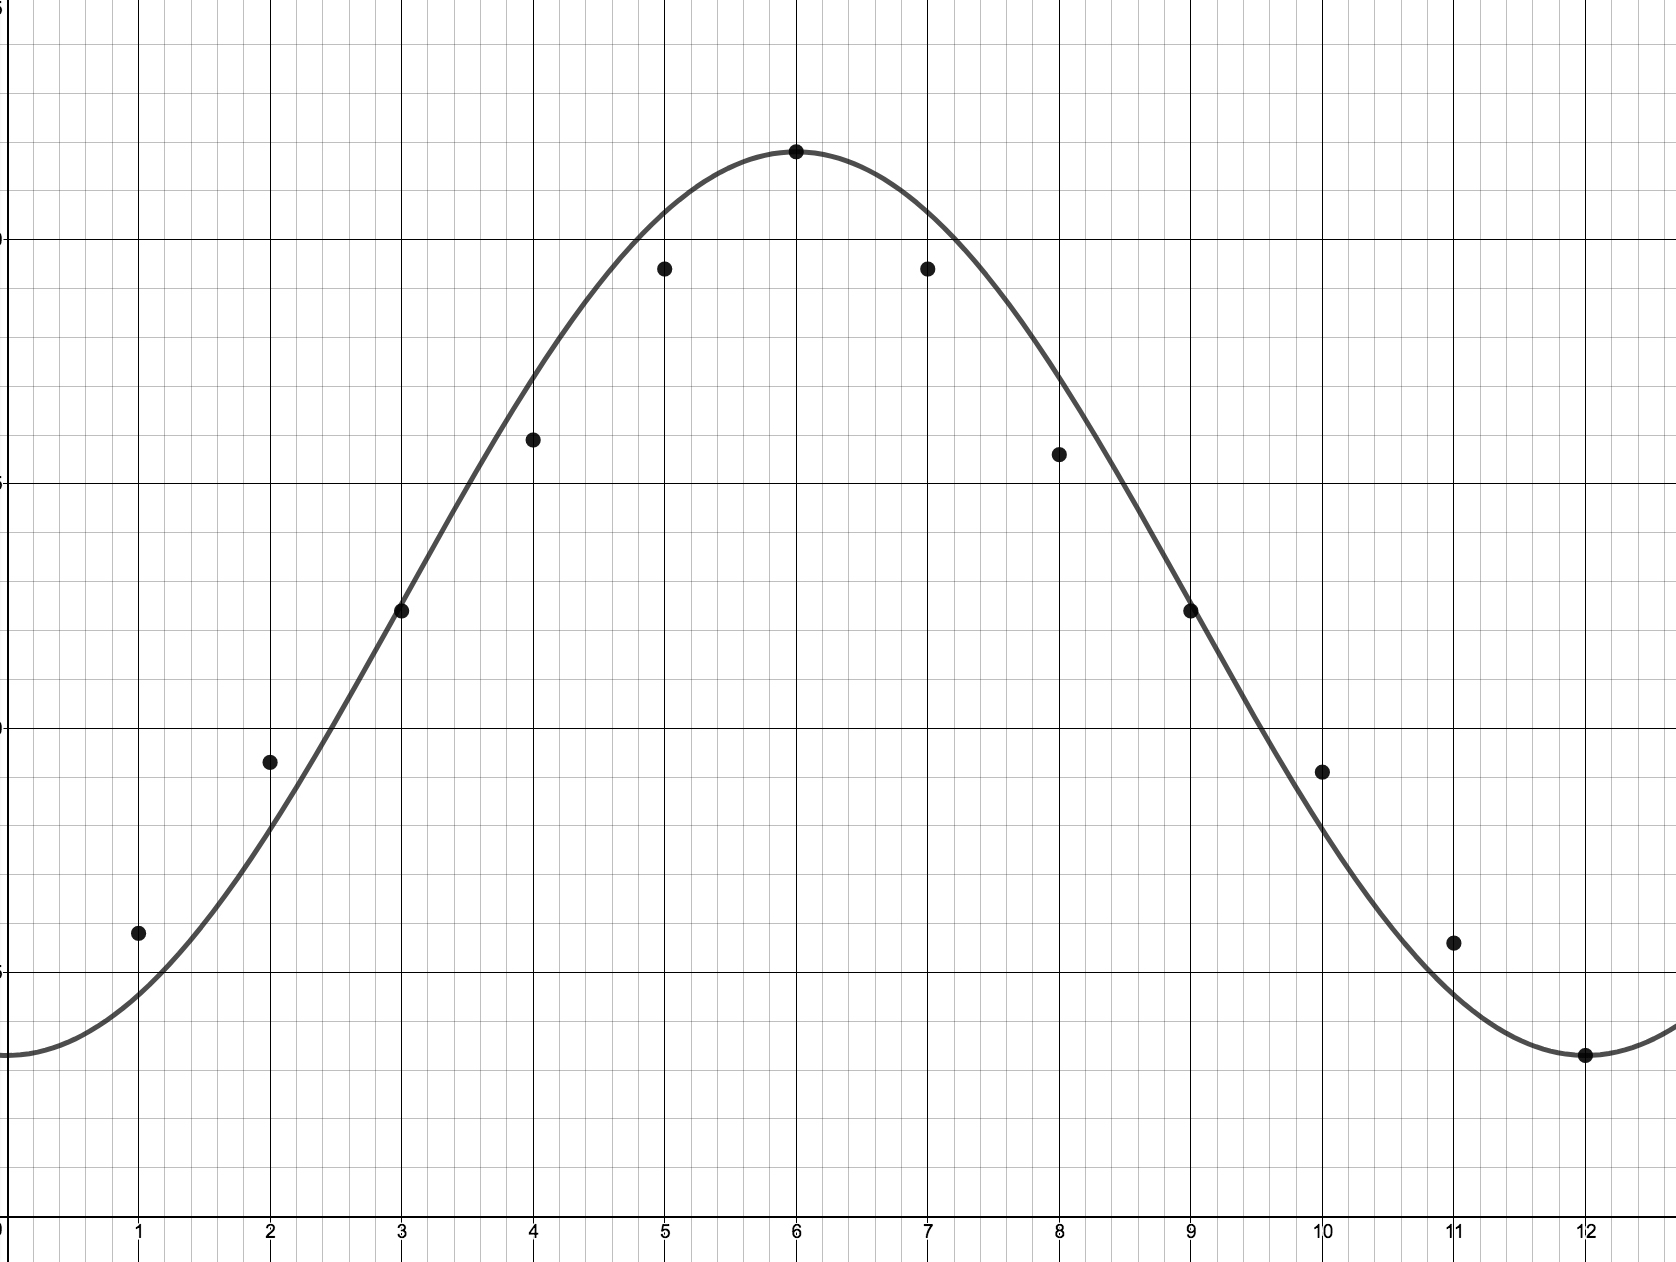
\includegraphics[height=2.5in]{./GraphsofSineandCosineGraphics/RoughFitDaylight.jpg}

\end{multicols}

\begin{multicols}{2}

Plotting the data.


Plotting the data long with $y=H(t)$


\end{multicols}

\end{center}

 
\item  Using  \href{https://www.desmos.com}{\underline{desmos}} to find a regression model produces $A \approx 8.36$ and $B \approx 12.06$, which closely match our answers from number \ref{roughsinusoidfit}. However, desmos calculates $\omega \approx -294.81$ and $\phi \approx -26.53$, which are far from our values $\omega = \frac{\pi}{6}$ and $\phi = -\frac{\pi}{2}$. 

\smallskip

Indeed, in Exercise \ref{graphdesmosregression}, we invite the reader to graph $y = 8.36 \sin(-294.81t  - 26.53) + 12.06$ using desmos.  At first glance, appears to be a solid gray rectangle. After zooming in, however, we see this rectangle is made up of literally hundreds of oscillations.  Though desmos boasts this regression as having an $R^{2}$ value of $0.9886$, meaning mathematically, this is a very good fit to the data, this curve doesn't model the real-world phenomenon of daylight hours in any sort of reasonable manner. 

\smallskip

Since we know the period of the sinusoid is 12 months, we set $\omega = \frac{\pi}{6}$ and ask desmos to run a regression for the remaining three parameters.   Desmos returns the values $A \approx -8.13$, $B \approx 12.5$, and $\phi \approx -4.70$, with an $R^{2}$ value of $0.987$,  so its regression curve is a much more reasonable $H(t) = -8.13 \sin\left(\frac{\pi}{6} t - 4.70\right)+ 12.5$.  Even though, at first glance, this curve appears much different from our solution to number \ref{roughsinusoidfit}, the we graph both functions below on the right and see they are very similar.\footnote{In Section \ref{MoreTrigonometricIdentities}, we can show how similar these two functions are analytically.  See Exercise \ref{twodaylightfunctions}.}  (Our solution to number \ref{roughsinusoidfit} is the darker of the two curves.)

\begin{center}

\begin{multicols}{2}
 

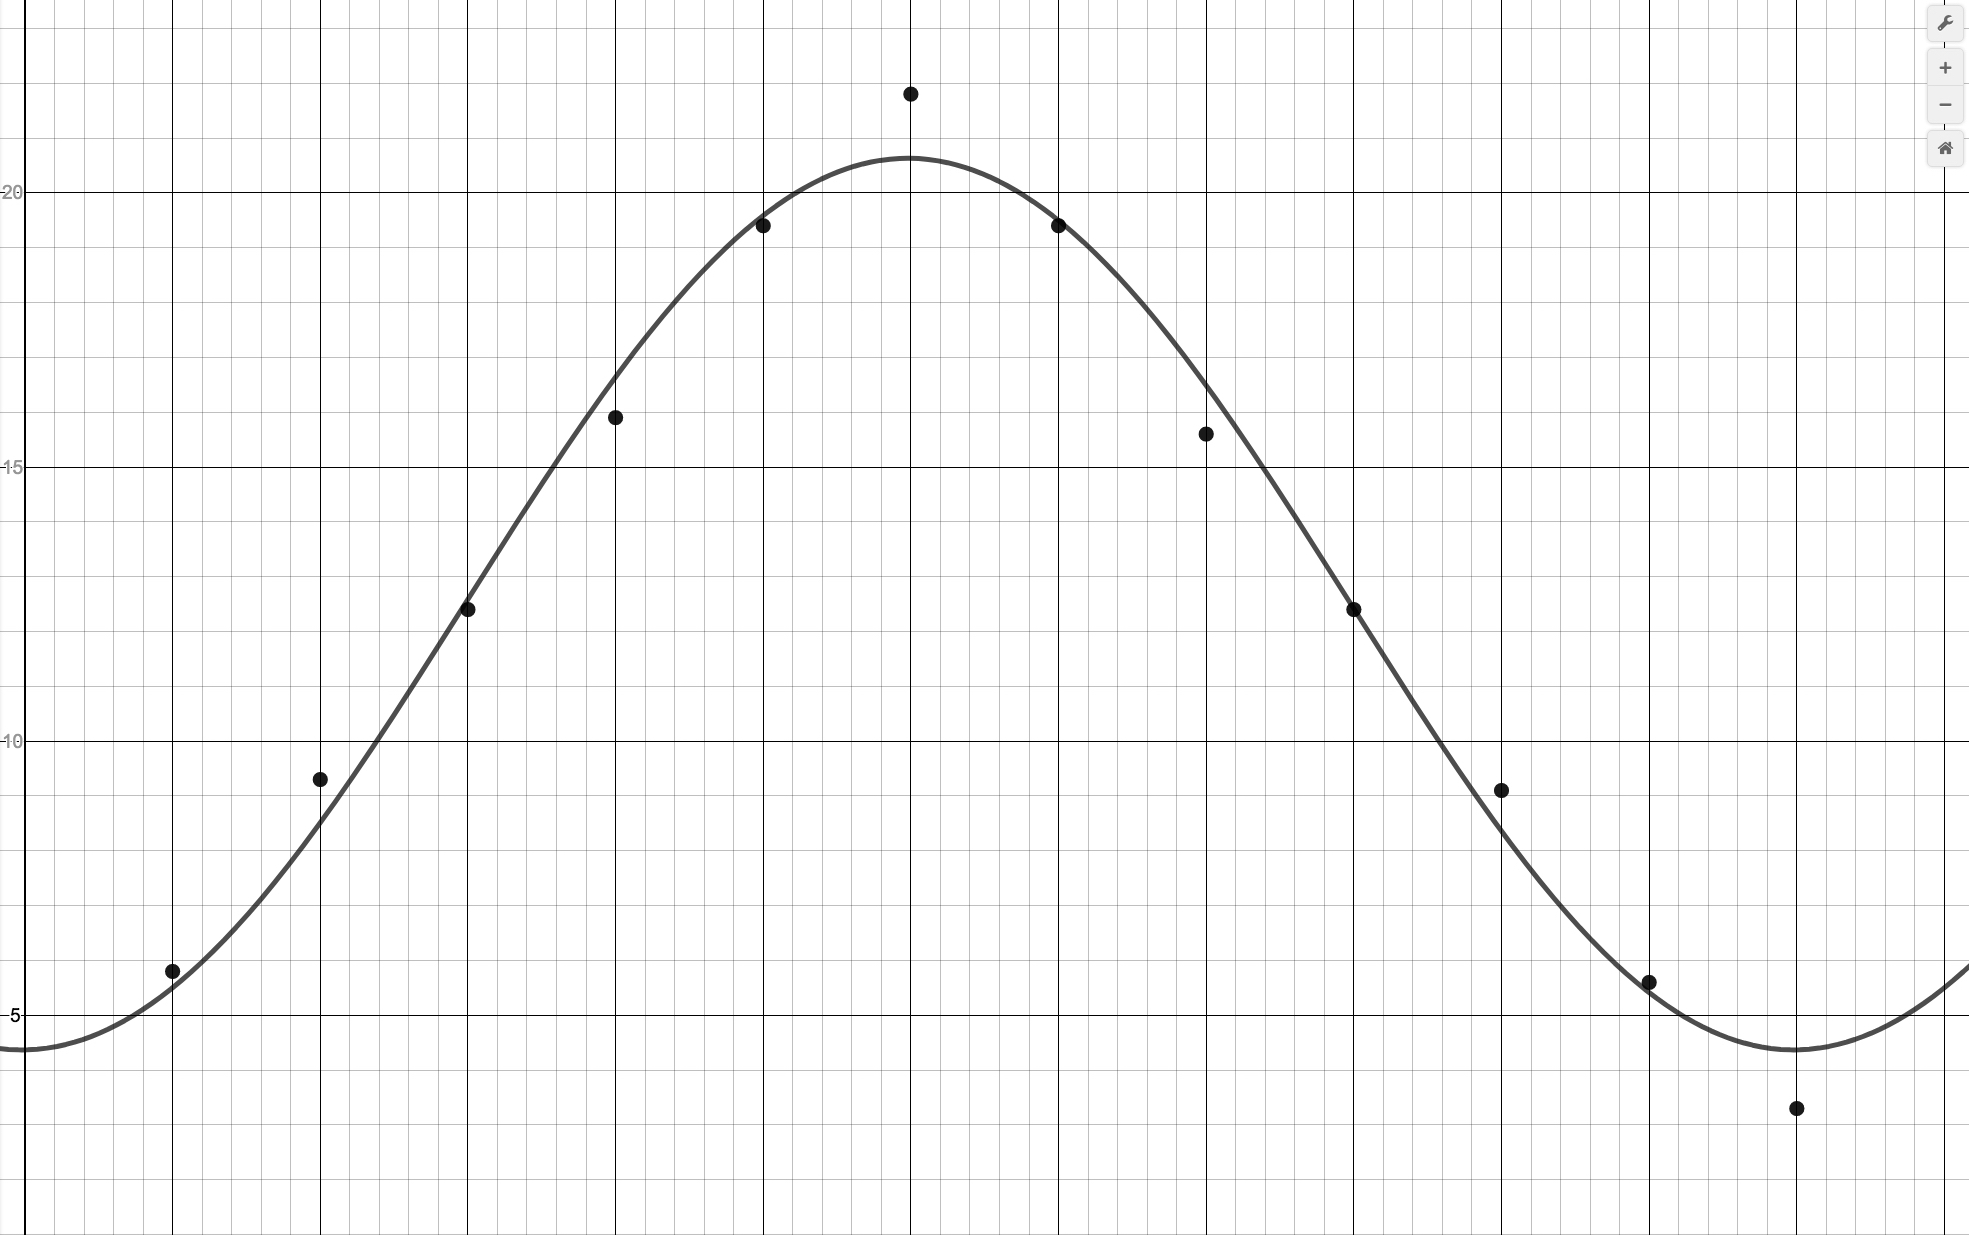
\includegraphics[width=2.75 in]{./GraphsofSineandCosineGraphics/desmos_regression.jpg}
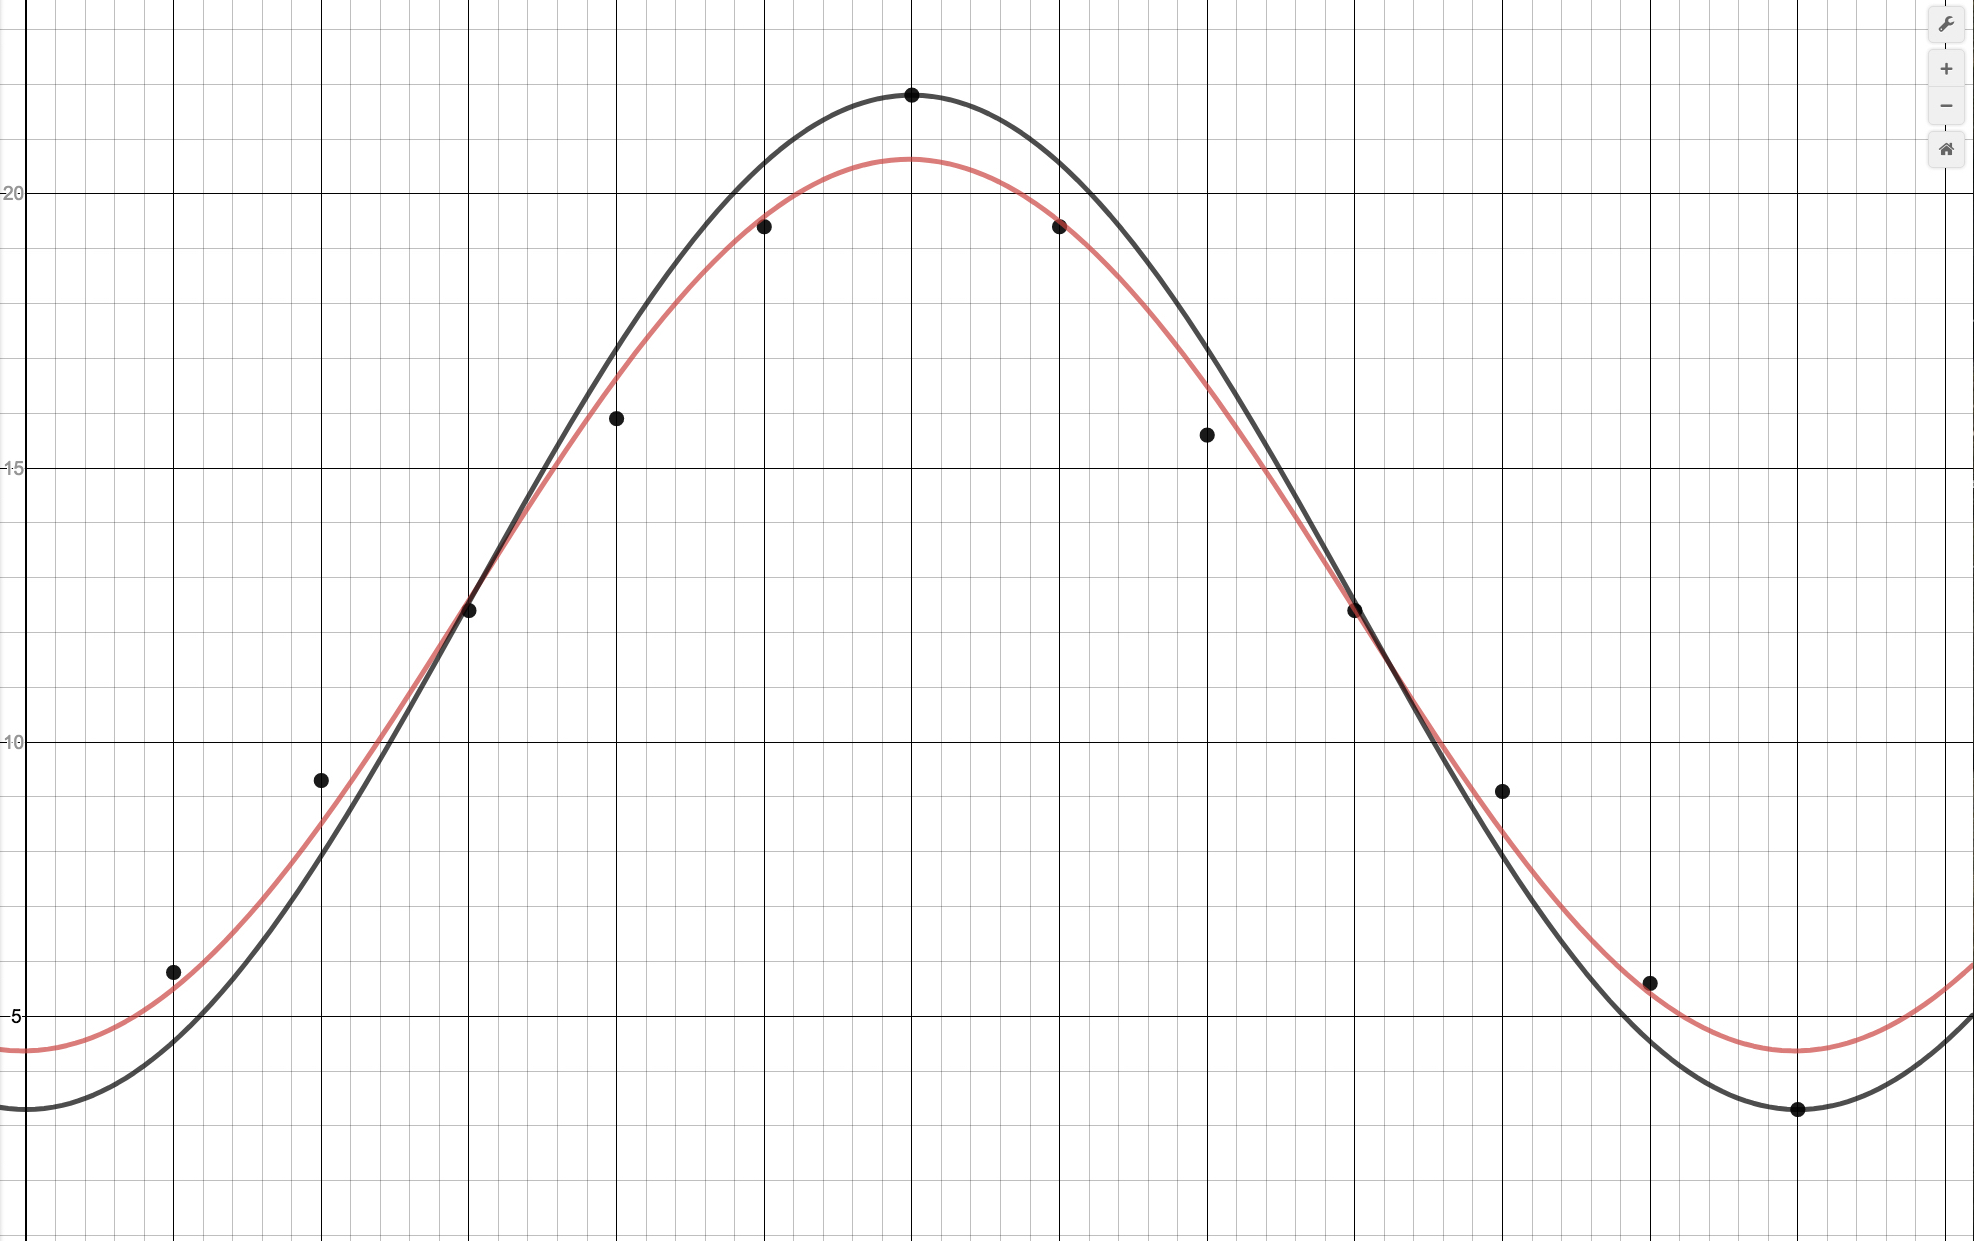
\includegraphics[width=2.75 in]{./GraphsofSineandCosineGraphics/both_daylight.jpg}
 

 
 \end{multicols}
 
 \begin{multicols}{2}

Plotting the desmos's regression curve.


Plotting both solutions.


\end{multicols}
 
 
 \end{center}
 
 \qed

\end{enumerate}

\end{ex}

The scenario described in Example \ref{sinusoidsunlight} is a typical example of where the circular functions are useful outside the context of angles or circular motion.  Indeed, sine and cosine functions are used extensively to model a wide range of periodic phenomena including signal analysis, wave physics, and even quantum mechanics.  We close this section discussing limits involving sine and cosine. 

\subsection{Limits involving Sine and Cosine}
\label{SineCosineLimits}

We've already stated as fact (but not proven) that $f(t) = \sin(t)$ and $g(t) = \cos(t)$ are continuous.  Per Definition \ref{continuousdefn}, this means that $\ds{\lim_{t \rightarrow a} \sin(t) = \sin(a)}$ and $\ds{\lim_{t \rightarrow a} \cos(t) = \cos(a)}$ for all real numbers, $a$.  This means, for instance, we can compute  $\ds{\lim_{t \rightarrow \pi} \cos(t) = \cos(\pi) = -1}$.  Per the discussion following Definition \ref{continuousdefn}, so long as we avoid the usual domain pitfalls, we can also compute:
 \[ \lim_{t \rightarrow \pi} \frac{2t \cos(t) - \sin(3t)}{\sqrt{\cos(2t)}} = \frac{2 \pi \cos(\pi) - \sin(3\pi)}{\sqrt{\cos(2\pi)}} = \frac{-2\pi - 0}{\sqrt{1}} = - 2\pi \]
 
 In the next example we investigate a few (similar looking) limits of sinusoids.
 
 \pagebreak
 
 \begin{ex}\label{sinusoidgraphs}  Investigate the following limits numerically, graphically, and analytically.
 
 \begin{multicols}{3}
 \begin{enumerate}
 
 \item $\ds{ \lim_{t \rightarrow 0}}$ $\sin\left( \frac{\pi}{t} \right)$ 
  \item $\ds{ \lim_{t \rightarrow 0}}$ $\sin\left( 10^{23} \, t \right)$
   \item $\ds{ \lim_{t \rightarrow 0}}$ $ \frac{\sin(t)}{t}$
   
   \end{enumerate}
   
   \end{multicols}
   
 {\bf Solution.}
 
\begin{enumerate}

\item   To analyze $\ds{ \lim_{t \rightarrow 0}}$ $\sin\left( \frac{\pi}{t} \right)$ numerically, we construct a table of values `near' $t = 0$ for $F(t) = \sin\left( \frac{\pi}{t} \right)$.  Choosing values such as $t = \pm 0.001$,  $t = \pm 0.01$, etc., we get  a list of `$0$'s. This result shouldn't be too surprising since in each of these cases, $\frac{\pi}{t}$ results in an integer multiple of $\pi$. However, the graph near $t=0$ (literally) paints a different picture.  The graph appears to wildly oscillate near $t=0$, suggesting that  $\ds{ \lim_{t \rightarrow 0}}$ $\sin\left( \frac{\pi}{t} \right)$ does not exist.

\begin{center}

 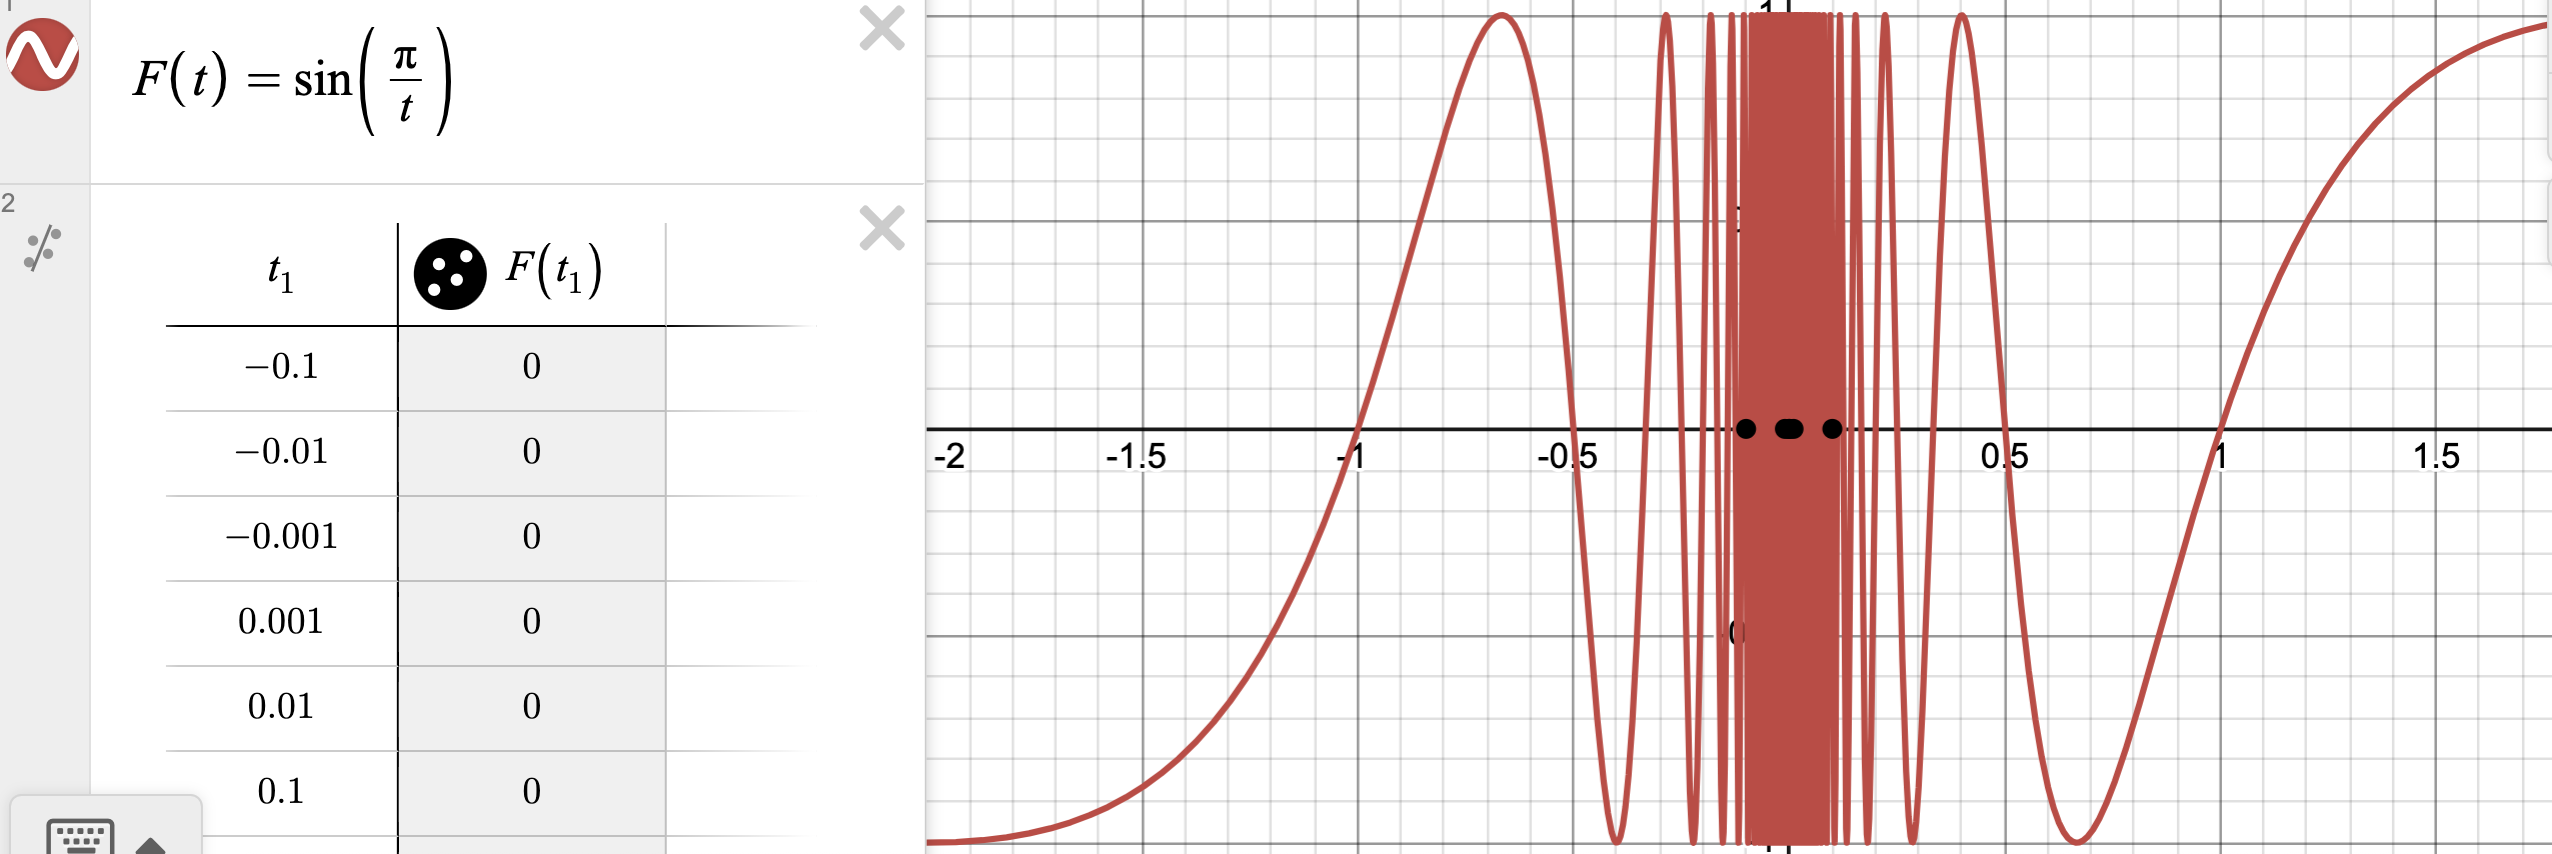
\includegraphics[width=6in]{./GraphsofSineandCosineGraphics/sinpiovert.png}
 
 \end{center}
 
 Indeed, as $t \rightarrow 0^{-}$, $\frac{\pi}{t} \rightarrow -\infty$ and as $t \rightarrow 0^{+}$, $\frac{\pi}{t} \rightarrow \infty$.  In other words, all of the infinite oscillations experienced by the standard sine function, $f(t) = \sin(t)$ as $t \rightarrow -\infty$ and as $t \rightarrow \infty$ are being brought  back to near  $t = 0$ in $F(t) = \sin\left( \frac{\pi}{t} \right)$.  Hence, $\ds{ \lim_{t \rightarrow 0}}$ $\sin\left( \frac{\pi}{t} \right)$ does not exist.


\item  We proceed as above to investigate $\ds{ \lim_{t \rightarrow 0}}$ $\sin\left( 10^{23} \, t \right)$.    A table and  a graph of  $F(t) = \sin \left( 10^{23} \, t\right)$  `near' $t = 0$ produces numerical and graphical noise.  Neither the table nor the graph suggest $\ds{\lim_{t \rightarrow 0} F(t)}$ exists.  However, we know  $F(t) = \sin \left( 10^{23} \, t\right)$ is a sinusoid with frequency $\omega = 10^{23}$.  Zooming in by a factor of $10^{23}$, we get one cycle of $F$ which suggests the limit is, in fact, $0$.

\begin{center}

\begin{tabular}{cc}


 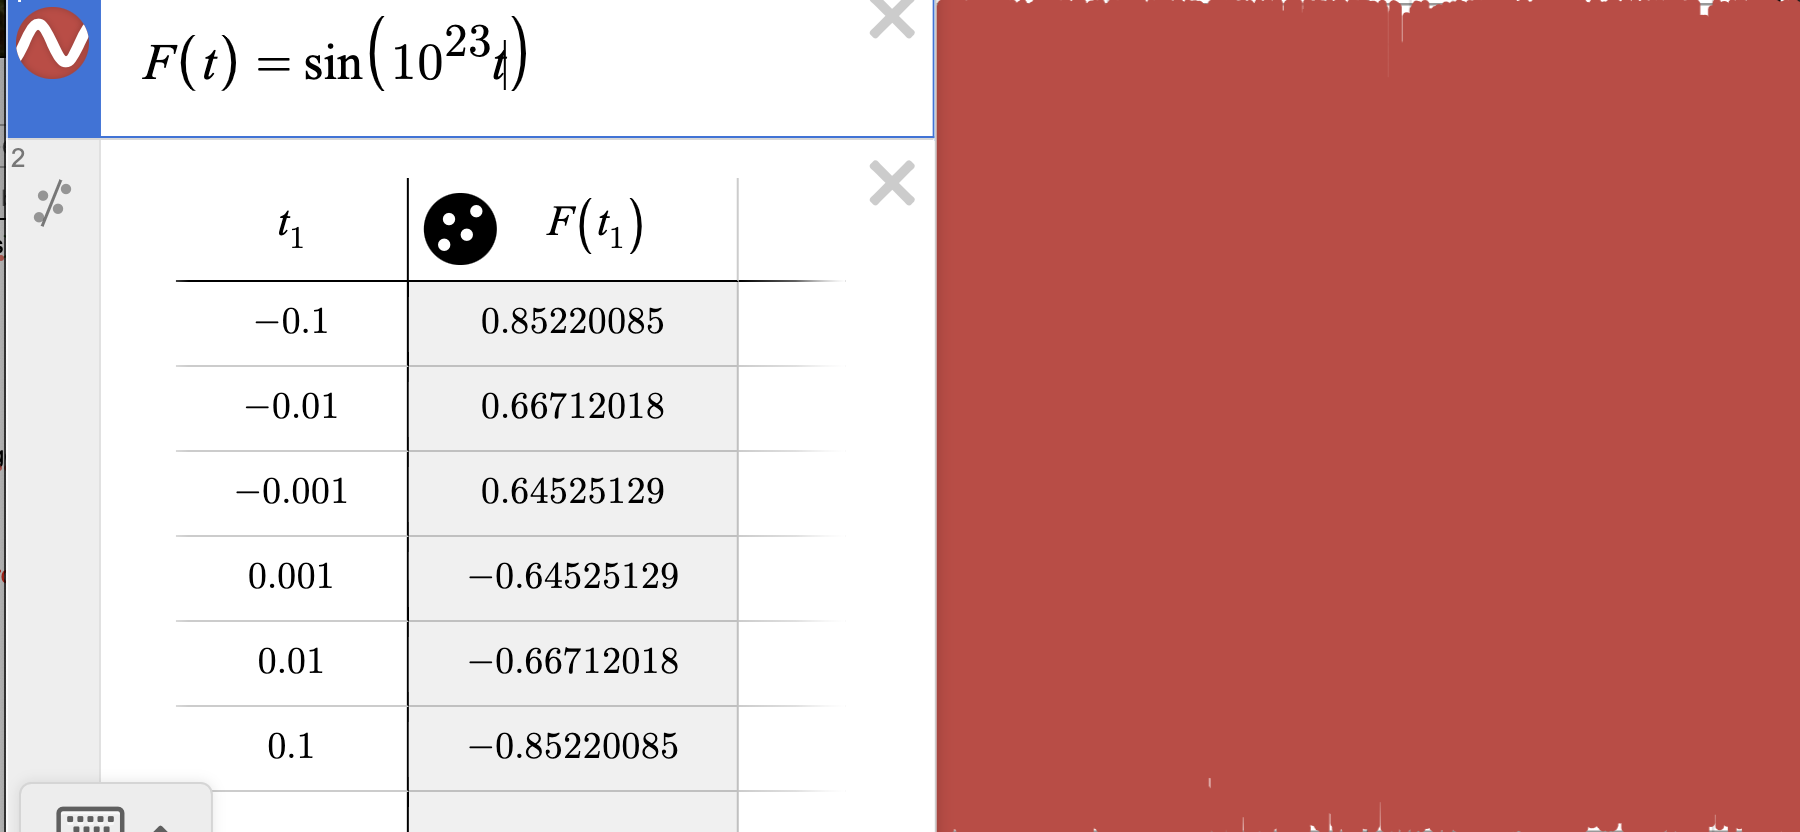
\includegraphics[width=3in]{./GraphsofSineandCosineGraphics/sine10^23tfar.png}  &    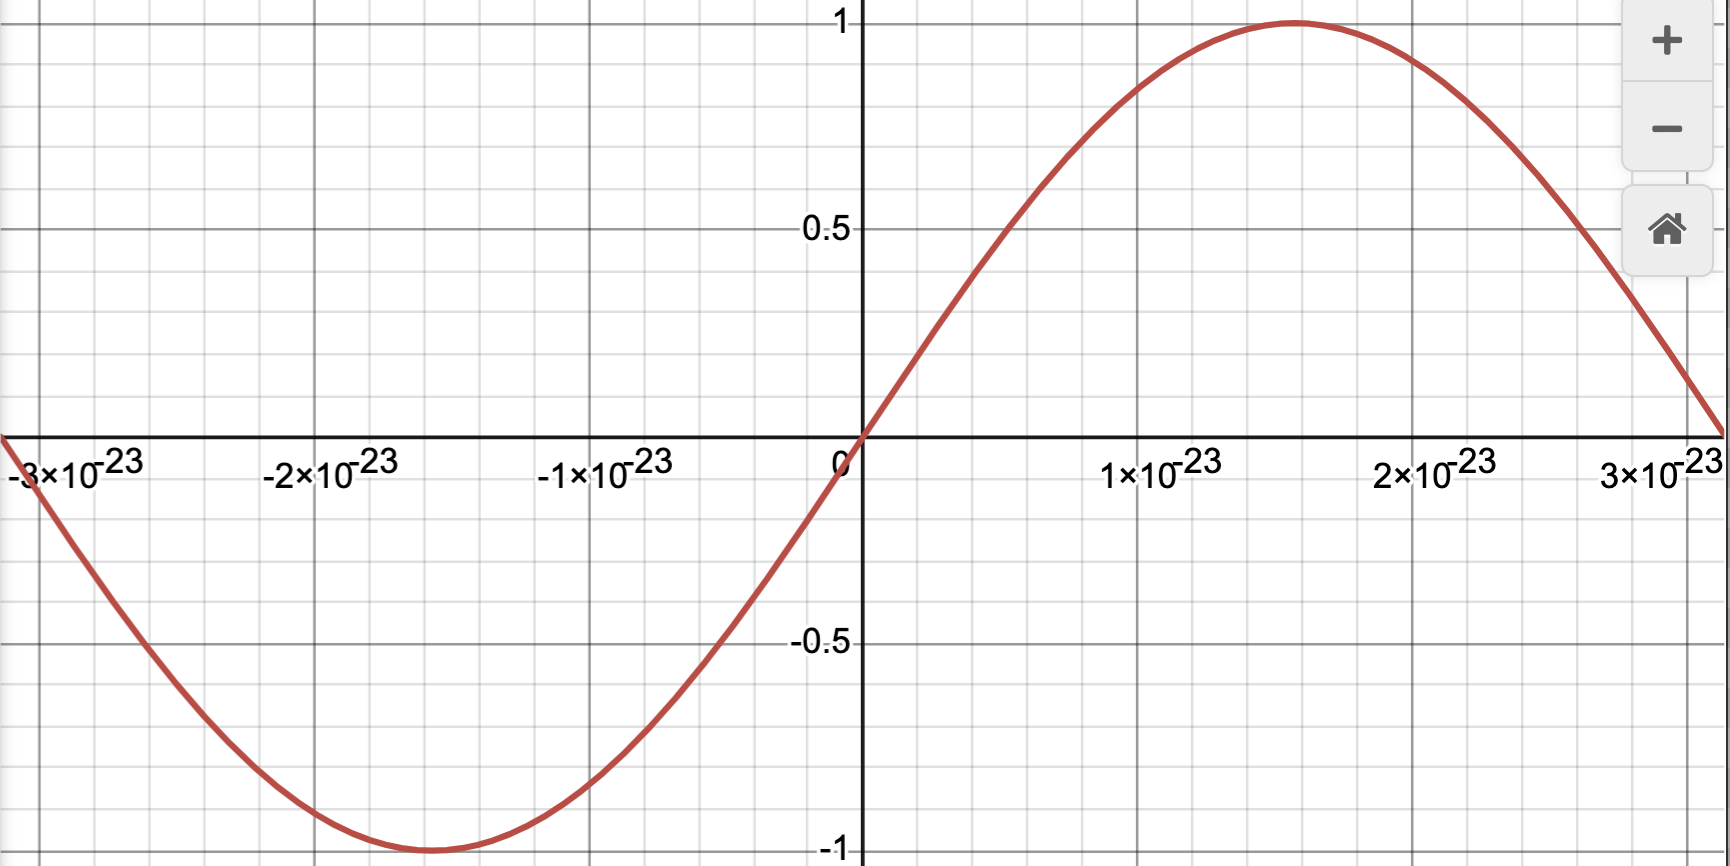
\includegraphics[width=3in]{./GraphsofSineandCosineGraphics/sine10^23tzoom.png}  \\
 
 $F(t) = \sin \left( 10^{23} \, t\right)$ `near' $t=0$ &  $F(t) = \sin \left( 10^{23} \, t\right)$ `nearer to ' $t=0$ \\
 
 \end{tabular}
 
\end{center}



Indeed, we know  $F(t) = \sin \left( 10^{23} \, t\right)$ is continuous, so $\ds{ \lim_{t \rightarrow 0}}$ $\sin\left( 10^{23} \, t \right) = \sin\left(10^{23} (0)) \right) = \sin(0) = 0$.   

\item  Next we investigate  $F(t) =  \frac{\sin(t)}{t}$ near $t=0$.   The table and graph both suggest   $\ds{ \lim_{t \rightarrow 0}}$ $ \frac{\sin(t)}{t} = 1$. 



\begin{center}

 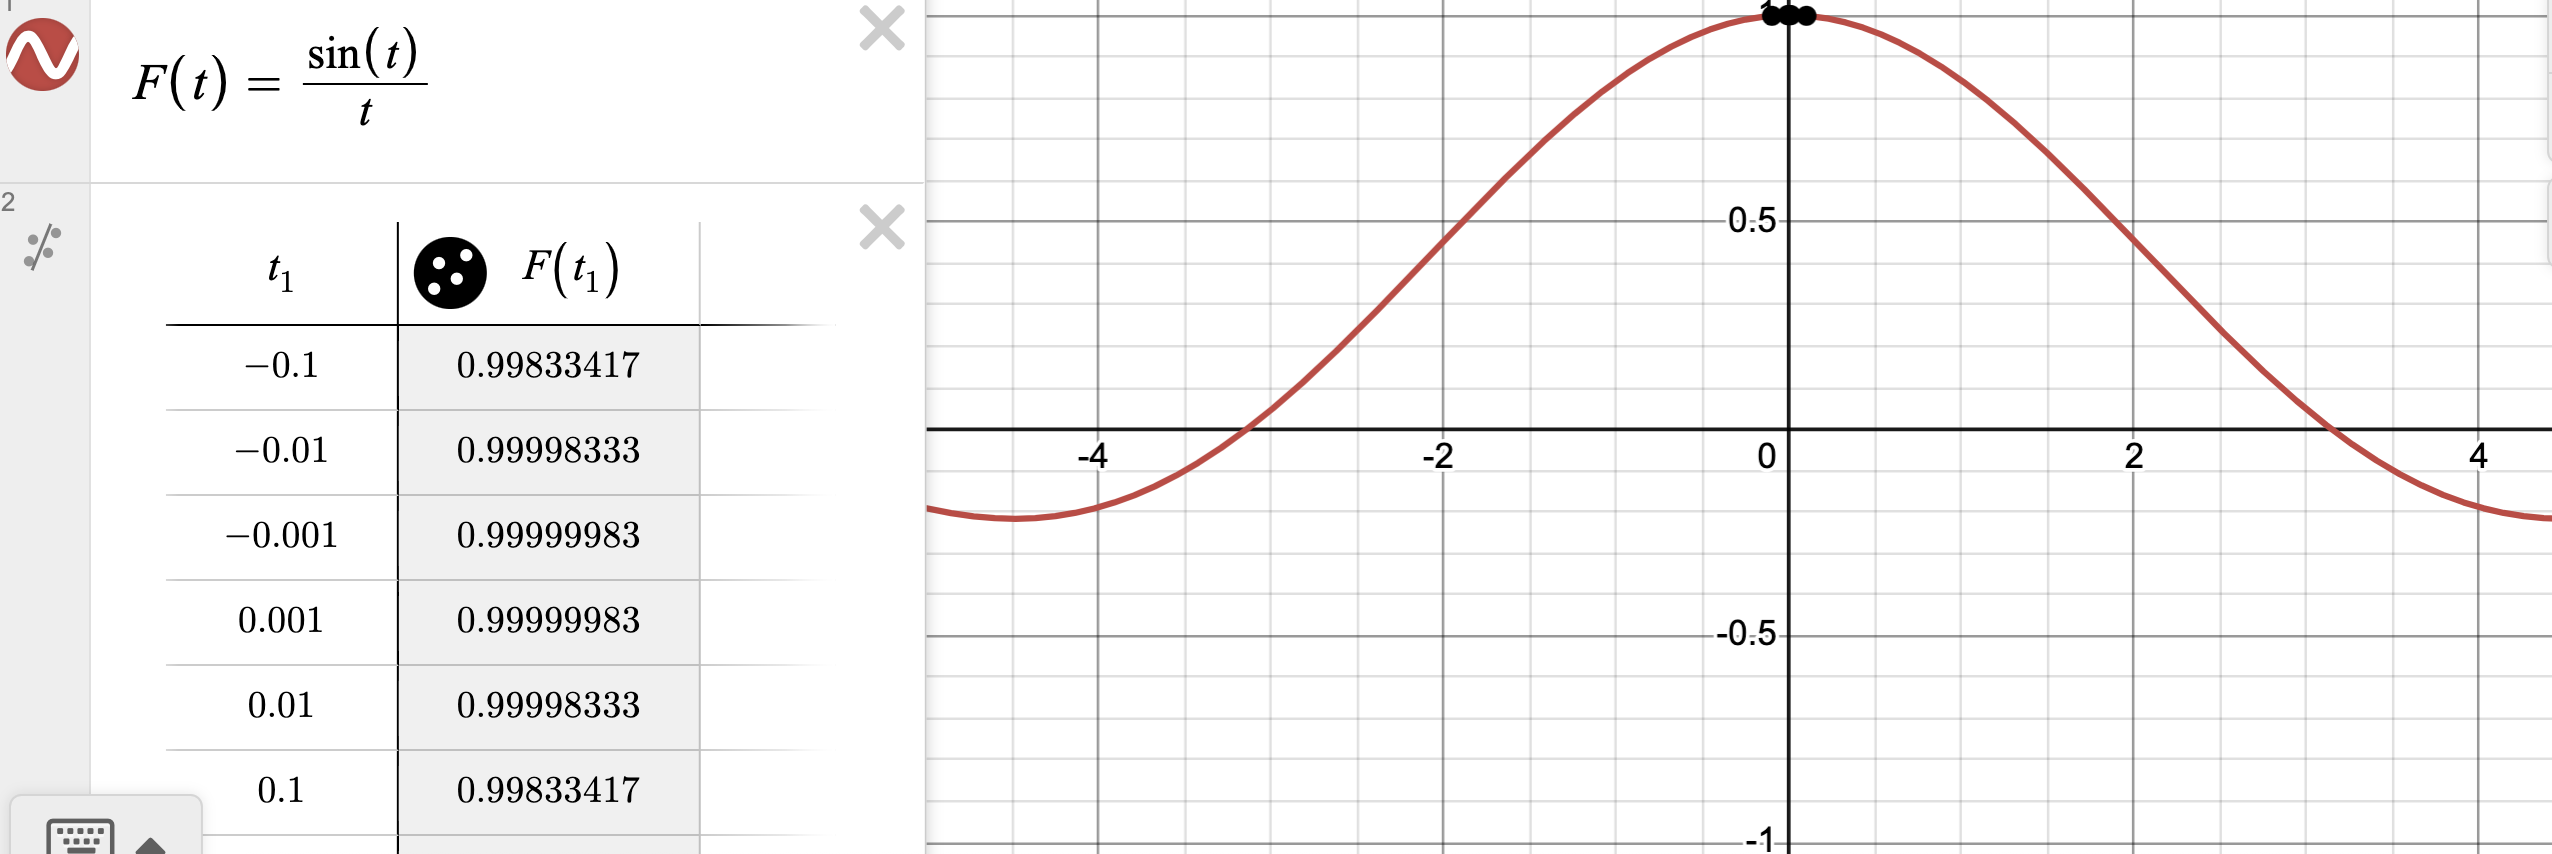
\includegraphics[width=6in]{./GraphsofSineandCosineGraphics/sintovert.png}
 
 \end{center}
 
 Attempting to analyze this limit analytically, we see that  $\ds{ \lim_{t \rightarrow 0}}$ $ \frac{\sin(t)}{t}$ produces the indeterminate form `$\frac{0}{0}$'.  At this stage, we do not have the tools to either prove or disprove our conjecture that  $\ds{ \lim_{t \rightarrow 0}}$ $ \frac{\sin(t)}{t} = 1$,  but we will soon, \footnote{See Exercises \ref{sintovertexercise1} through \ref{sintovertexercise3} in Section \ref{TheOtherCircularFunctions}.} so stay tuned!  \qed

\end{enumerate}

\end{ex}



\newpage

\subsection{Exercises}

\documentclass{ximera}

\begin{document}
	\author{Stitz-Zeager}
	\xmtitle{TITLE}
\mfpicnumber{1} \opengraphsfile{ExercisesforGraphsofSineandCosine} % mfpic settings added 


In Exercises \ref{sinecosinegraphfirst} - \ref{sinecosinegraphlast}, graph one cycle of the given function.  State the period, amplitude, phase shift and vertical shift of the function.

\begin{multicols}{3}

\begin{enumerate}

\item $f(t) = 3\sin(t)$ \label{sinecosinegraphfirst}
\item $g(t) = \sin(3t)$
\item $h(t)  = -2\cos(t)$

\setcounter{HW}{\value{enumi}}

\end{enumerate}

\end{multicols}

\begin{multicols}{3}

\begin{enumerate}

\setcounter{enumi}{\value{HW}}

\item $f(t)  = \cos \left( t - \frac{\pi}{2} \right)$
\item $g(t)  = -\sin \left( t + \frac{\pi}{3} \right)$
\item $h(t) = \sin(2t - \pi)$ \vphantom{$\left( \frac{\pi}{2} \right)$}

\setcounter{HW}{\value{enumi}}

\end{enumerate}

\end{multicols}

\begin{multicols}{3}

\begin{enumerate}

\setcounter{enumi}{\value{HW}}

\item $f(t)  = -\frac{1}{3}\cos \left( \frac{1}{2}t + \frac{\pi}{3} \right)$
\item $g(t) = \cos (3t - 2\pi) + 4$ \vphantom{$\left( \frac{1\pi}{2} \right)$}
\item $h(t)  = \sin \left( -t - \frac{\pi}{4} \right) - 2$ \vphantom{$\left( \frac{1\pi}{2} \right)$}

\setcounter{HW}{\value{enumi}}

\end{enumerate}

\end{multicols}

\begin{multicols}{3}

\begin{enumerate}

\setcounter{enumi}{\value{HW}}

\item $f(t) = \frac{2}{3} \cos \left( \frac{\pi}{2} - 4t \right) + 1$
\item $g(t) = -\frac{3}{2} \cos \left( 2t + \frac{\pi}{3} \right) - \frac{1}{2}$
\item $h(t) = 4\sin (-2\pi t + \pi)$ \vphantom{$\left( \frac{1\pi}{2} \right)$}  \label{sinecosinegraphlast}

\setcounter{HW}{\value{enumi}}

\end{enumerate}

\end{multicols}

In Exercises \ref{fitsinecosinefirst} - \ref{fitsinecosinelast},  a sinusoid is graphed. Find a formula for the sinusoid in the form $S(t) = A \sin(\omega t + \phi) + B$ and $C(t) = A \cos(\omega t + \phi) + B$.  Select $\omega$ so  $\omega > 0$. Check your answer by graphing.

\begin{multicols}{2}
\begin{enumerate}
\setcounter{enumi}{\value{HW}}

\item $~$   \label{fitsinecosinefirst}  %$S(t) = 4 \sin \left(t + \frac{\pi}{4} \right)$, $C(t) = 4 \cos \left(t - \frac{\pi}{4} \right)$

\begin{mfpic}[16]{-5}{5}{-5}{5}
\tlabel[cc](5,-0.30){\scriptsize $t$}
\tlabel[cc](0.25,5){\scriptsize $y$}
\axes
\xmarks{-4 step 1 until 4}
\ymarks{-4 step 1 until 4}
\point[4pt]{(-3.927, 0), (-2.356, -4), (-0.7854, 0), (0.7854, 4), (2.356, 0)}
\tlabel[cc](-3, 0.5){ \scriptsize $\left( -\frac{5\pi}{4}, 0 \right)$}
\tlabel[cc](-2.356, -4.5){ \scriptsize $\left( -\frac{3\pi}{4}, -4 \right)$}
\gclear \tlabelrect(0.25, -0.6){ \scriptsize $\left( -\frac{\pi}{4}, 0 \right)$ \vphantom{$\dfrac{5}{2}$}}
\tlabel[cc](0.9, 4.5){\scriptsize $\left( \frac{\pi}{4}, 4 \right)$}
\tlabel[cc](3.25, 0.5){ \scriptsize $\left( \frac{3\pi}{4}, 4 \right)$}
\tlpointsep{4pt}
%\axislabels {x}{{$\frac{\pi}{2}$} 1.5708, {$\pi$} 3.1416, {$\frac{3\pi}{2}$} 4.7124, {$2\pi$} 6.2832}
%\axislabels {y}{{$-3$} -3, {$3$} 3}
\penwd{1.25pt}
\arrow \reverse \arrow \function{-5, 5,  0.1}{4*sin(x+(pi/4))}
\end{mfpic}   


\item$~$     % $S(t) = -3 \sin(t) + 3$, $C(t) = -3 \cos\left(t - \frac{\pi}{2}\right) + 3$

\begin{mfpic}[16]{-6}{6}{-1}{9}
\tlabel[cc](6,-0.30){\scriptsize $t$}
\tlabel[cc](0.25,9){\scriptsize $y$}
\axes
\xmarks{-5 step 1 until 5}
\ymarks{1 step 1 until 8}
\point[4pt]{(-4.712, 0), (-1.571, 6), (0,3), (1.571, 0), (4.712, 6)}
\tlabel[cc](-4.712, -0.75){\scriptsize $\left( -\frac{3\pi}{2}, 0 \right)$}
\tlabel[cc](-1.571, 6.5){\scriptsize $\left( -\frac{\pi}{2}, 6 \right)$}
\tlabel[cc](0.75, 3){ \scriptsize $\left(0, 3 \right)$}
\tlabel[cc](4.712, 6.5){\scriptsize $\left( \frac{3 \pi}{2}, 6 \right)$}
\tlabel[cc](1.571, -0.75){\scriptsize $\left( \frac{\pi}{2}, 0 \right)$}
\tlpointsep{4pt}
%\axislabels {x}{{$\frac{\pi}{2}$} 1.5708, {$\pi$} 3.1416, {$\frac{3\pi}{2}$} 4.7124, {$2\pi$} 6.2832}
%\axislabels {y}{{$-3$} -3, {$3$} 3}
\penwd{1.25pt}
\arrow \reverse \arrow \function{-6, 6,  0.1}{3- 3*sin(x)}
\end{mfpic}  

\setcounter{HW}{\value{enumi}}
\end{enumerate}
\end{multicols}

\begin{multicols}{2}
\begin{enumerate}
\setcounter{enumi}{\value{HW}}

\item $~$    %$S(t) = 3 \sin \left( 2t - \frac{\pi}{3} \right)$, $C(t) = 3 \cos \left( 2t - \frac{5\pi}{6} \right)$

\begin{mfpic}[15]{-6}{6}{-5}{5}
\tlabel[cc](6,-0.30){\scriptsize $t$}
\tlabel[cc](0.25,5){\scriptsize $y$}
\axes
\xmarks{-5 step 1 until 5}
\ymarks{-4 step 1 until 4}
\point[4pt]{(-4.974, 3), (-4.189, 0), (-3.403, -3), (-2.618, 0), (-1.832, 3), (-1.047, 0), (-0.2618, -3), (0.5236, 0), (1.309, 3), (2.094, 0), (2.8880, -3), (3.665, 0), (4.45, 3), (5.236, 0)}
\tlabel[cc](-4.974, 3.75){ \scriptsize $\left( -\frac{19 \pi}{12}, 3 \right)$}
\tlabel[cc](-3.403, -3.75){ \scriptsize $\left( -\frac{13 \pi}{12}, -3 \right)$}
\tlabel[cc] (-1.832, 3.75){ \scriptsize $\left( -\frac{7 \pi}{12}, 3 \right)$}
\gclear \tlabelrect(0, -3.75){ \scriptsize $\left( -\frac{\pi}{12}, -3 \right)$}
\tlabel[cc] (1.309, 3.75){ \scriptsize $\left( \frac{5 \pi}{12}, 3 \right)$}
\tlabel[cc](2.880, -3.75){ \scriptsize $\left( \frac{11 \pi}{12}, -3 \right)$}
\tlabel[cc] (4.45, 3.75){ \scriptsize $\left( \frac{17 \pi}{12}, 3 \right)$}

\tlpointsep{4pt}
%\axislabels {x}{{$\frac{\pi}{2}$} 1.5708, {$\pi$} 3.1416, {$\frac{3\pi}{2}$} 4.7124, {$2\pi$} 6.2832}
%\axislabels {y}{{$-3$} -3, {$3$} 3}
\penwd{1.25pt}
\arrow \reverse \arrow \function{-6, 5.5,  0.1}{3*sin((2*x)-(pi/3))}
\end{mfpic}   


\item$~$     \label{fitsinecosinelast}  % $S(t) =  \frac{7}{2} \sin(\pi t) + \frac{1}{2}$, $C(t) = \frac{7}{2} \cos\left(\pi t \frac{\pi}{2} \right) + \frac{1}{2}$

\begin{mfpic}[22][15]{-5}{5}{-5}{5}
\tlabel[cc](5,-0.30){\scriptsize $t$}
\tlabel[cc](0.25,5){\scriptsize $y$}
\axes
\xmarks{-4 step 1 until 4}
\ymarks{-4 step 1 until 4}
\point[4pt]{ (-4, 0.5), (-3.5, 4), (-3, 0.5), (-2.5, -3), (-2, 0.5), (-1.5, 4), (-1, 0.5), (-0.5, -3), (0, 0.5), (0.5, 4), (1, 0.5), (1.5,-3), (2, 0.5), (2.5,4), (3, 0.5), (3.5,-3), (4, 0.5) }
%\tlabel[cc](-4.5, -3.5){\scriptsize $(-4.5, -3)$}
\tlabel[cc](-3.5, 4.5){\scriptsize $(-3.5, 4)$}
\tlabel[cc](-2.5, -3.5){\scriptsize $(-2.5, -3)$}
\tlabel[cc](-1.5, 4.5){\scriptsize $(-1.5, 4)$}
%\tlabel[cc](-0.5, -3.5){\scriptsize $(-0.5, -3)$}
\gclear \tlabelrect(0.75, 4.5){\scriptsize $(0.5, 4)$}
\tlabel[cc](1.5, -3.5){\scriptsize $(1.5, -3)$}
\tlabel[cc](2.5, 4.5){\scriptsize $(2.5, 4)$}
%\tlabel[cc](2.5, -3.5){\scriptsize $(2.5, -3)$}
%\tlabel[cc](4.5, 4.5){\scriptsize $(4.5, 4)$}

\tlpointsep{4pt}
%\axislabels {x}{{$\frac{\pi}{2}$} 1.5708, {$\pi$} 3.1416, {$\frac{3\pi}{2}$} 4.7124, {$2\pi$} 6.2832}
%\axislabels {y}{{$-3$} -3, {$3$} 3}
\penwd{1.25pt}
\arrow \reverse \arrow \function{-4.25, 4.25,  0.1}{(3.5*sin(pi*x))+0.5}
\end{mfpic}   

\setcounter{HW}{\value{enumi}}
\end{enumerate}
\end{multicols}


\begin{enumerate}
\setcounter{enumi}{\value{HW}}

\item  Use the graph of  $S(t) = 4 \sin(t)$ to graph each of the following functions. State the period of each.

\begin{multicols}{2}

\begin{enumerate}

\item $f(t) = | 4 \sin(t)|$

\item $g(t) = \sqrt{4 \sin(t)}$

\end{enumerate}
\end{multicols}


\setcounter{HW}{\value{enumi}}
\end{enumerate}

In Exercises \ref{exploregraphsfirst} - \ref{exploregraphslast}, use a graphing utility to help you and your classmates discuss the given questions.


\begin{enumerate}

\setcounter{enumi}{\value{HW}}

\item  Graph $f(t) = \cos(3t) + \sin(t)$.  Is this function periodic?  If so, what is the period? \label{exploregraphsfirst}

\smallskip

\item  Graph $f(t) = t \sin(t)$ along with  $y = \pm t$. What do you notice? 

\smallskip

\item  Graph $f(t) = \frac{\sin(t)}{t}$ along with  $y = \pm \frac{1}{t}$.   What do you notice?

\begin{enumerate}

\item What appears to be $\ds{\lim_{t \rightarrow \infty} f(t)}$?    Interpret your answer graphically.

\smallskip

\item  Use the Squeeze Theorem, Theorem \ref{squeezeth} from Section \ref{Sequences} to prove your claim.  

\smallskip

\textbf{HINT:}  Since $-1 \leq \sin(t) \leq 1$, for $t>0$, $-\frac{1}{t} \leq \frac{\sin(t)}{t} \leq \frac{1}{t}$ \ldots

\end{enumerate}

\smallskip


\item  Graph $f(t) = \cos\left(\frac{1}{t}\right)$.  

\begin{enumerate}

\item Investigate  $\ds{\lim_{t \rightarrow 0} f(t)}$.  Does $\ds{\lim_{t \rightarrow 0} f(t)}$ exist?  Why or why not?

\smallskip

\item  Determine $\ds{\lim_{t \rightarrow \infty} f(t)}$ and interpret your answer graphically.

\end{enumerate}

\smallskip

\item  Graph $f(t) = e^{-0.1t} \left( \cos(2t) + \sin(2t)\right)$ along with $y = \pm 2 \, e^{-0.1t}$. What do you notice?  \label{exploregraphslast}

\begin{enumerate}

\item What appears to be $\ds{\lim_{t \rightarrow \infty} f(t)}$?   Interpret your answer graphically.

\smallskip

\item  Use the Squeeze Theorem, Theorem \ref{squeezeth} from Section \ref{Sequences} to prove your claim.  

\smallskip

\textbf{HINT:}  Since $-1 \leq \cos(2t) \leq 1$ and $-1 \leq \sin(2t) \leq 1$, $-2 \leq \cos(2t) + \sin(2t) \leq 2$.  

\smallskip

Hence, $-2 e^{-0.1t} \leq e^{-0.1t} \left( \cos(2t) + \sin(2t)\right) \leq 2e^{-0.1t}$ \ldots

\end{enumerate}

\smallskip


\setcounter{HW}{\value{enumi}}

\end{enumerate}

\begin{enumerate}

\setcounter{enumi}{\value{HW}}

\item Show every constant function $f$ is periodic by explaining why $f(x + 117) = f(x)$ for all real numbers $x$. Then show that $f$ has no period by showing that you cannot find a \emph{smallest} number $p$ such that $f(x + p) = f(x)$ for all real numbers $x$.  

\smallskip

Said differently, show that $f(x + p) = f(x)$ for all real numbers $x$ for ALL values of $p > 0$, so no smallest value exists to satisfy the definition of `period'.

\setcounter{HW}{\value{enumi}}

\end{enumerate}

\begin{enumerate}

\setcounter{enumi}{\value{HW}}

\item  The sounds we hear are made up of mechanical waves.  The note `A' above the note `middle C' is a sound wave with ordinary frequency $f = 440$ Hertz $= 440 \frac{\text{cycles}}{\text{second}}$.  Find a sinusoid which models this note, assuming that the amplitude is $1$ and the phase shift is $0$.

\item The voltage $V$ in an alternating current source has amplitude $220 \sqrt{2}$ and ordinary frequency $f = 60$ Hertz.  Find a sinusoid which models this voltage.  Assume that the phase is $0$.


\item \label{heightlondoneye} The \href{http://en.wikipedia.org/wiki/London_Eye}{\underline{London Eye}} is a popular tourist attraction in London, England and is one of the largest Ferris Wheels in the world.  It has a diameter of 135 meters and makes one revolution (counter-clockwise) every 30 minutes.  It is constructed so that the lowest part of the Eye reaches ground level, enabling passengers to simply walk on to, and off of, the ride.  Find a sinsuoid which models the height $h$ of the passenger above the ground in meters $t$ minutes after they board the Eye at ground level.

\item \label{leftrightlondoneye} On page \pageref{equationsforcircularmotion} in Section \ref{cosinesinebeyond}, we found the $x$-coordinate of counter-clockwise motion on a circle of radius $r$ with angular frequency $\omega$ to be $x = r\cos(\omega t)$, where $t=0$ corresponds to the point $(r,0)$.  Suppose we are in the situation of Exercise \ref{heightlondoneye} above.  Find a sinsusoid which models the horizontal \textit{displacement} $x$ of the passenger from the center of the Eye in meters $t$ minutes after they board the Eye.  Here we take $x(t) > 0$ to mean the passenger is to the \textit{right} of the center, while $x(t) < 0$ means the passenger is to the \textit{left} of the center.

\item  In Exercise \ref{yoyotrick} in Section \ref{RadianMeasure}, we introduced the yo-yo trick `Around the World' in which a yo-yo is thrown so it sweeps out a vertical circle.  As in that exercise, suppose the yo-yo string is 28 inches and it completes one revolution in 3 seconds.  If the closest the yo-yo ever gets to the ground is 2 inches, find a sinsuoid which models the height $h$ of the yo-yo above the ground in inches $t$ seconds after it leaves its lowest point.



\item  Consider the pendulum below.  Ignoring air resistance, the angular displacement of the pendulum from the vertical position, $\theta$, can be modeled as a sinusoid.\footnote{Provided $\theta$ is kept `small.'  Carl remembers the `Rule of Thumb' as being $20^{\circ}$ or less.  Check with your friendly neighborhood physicist to make sure.}


\begin{center}

\begin{mfpic}[15]{-3}{3}{-5}{1}
\polyline{(0,0), (0,-5)}
\dashed \polyline{(0,0), (2.5, -4.33)}
\arrow \parafcn{275, 295, 5}{4*dir(t)}
\tlabel[cc](1.29, -4.83){$\theta$}
\hatchcolor[gray]{.7}
\lhatch \rect{(-3,0), (3,1)}
\fillcolor[gray]{.7} 
\gfill \circle{(0,-5),0.25}
\gfill \circle{(2.5, -4.33),0.20}
\penwd{1.025}
\circle{(0,-5),0.25}
\circle{(2.5, -4.33),0.25}
\rect{(-3,0), (3,1)}
\end{mfpic} 
\end{center}

The amplitude of the sinusoid is the same as the initial angular displacement, $\theta_{\text{\tiny $0$}}$, of the pendulum and the  period of the motion is given by

\[T = 2\pi \sqrt{\dfrac{\ell}{g}}\]

where $\ell$ is the length of the pendulum and $g$ is the acceleration due to gravity.

\begin{enumerate}

\item  Find a sinusoid which gives the angular displacement $\theta$ as a function of time, $t$. Arrange things so $\theta(0) = \theta_{\text{\tiny $0$}}$.

\item  In Exercise \ref{pendulumproblem} section \ref{RootRadicalFunctions}, you found the length of the pendulum needed in Jeff's antique Seth-Thomas clock to ensure the period of the pendulum is $\frac{1}{2}$ of a second. Assuming the initial displacement of the pendulum is $15^{\circ}$, find a sinusoid which models the displacement of the pendulum $\theta$ as a function of time, $t$, in seconds. 

\end{enumerate}



\item  The table below lists the average temperature of Lake Erie as measured in Cleveland, Ohio on the first of the month for each month during the years 1971 -- 2000.\footnote{See this website: \href{http://www.erh.noaa.gov/cle/climate/cle/normals/laketempcle.html}{\underline{http://www.erh.noaa.gov/cle/climate/cle/normals/laketempcle.html}.}}  For example,   $t=3$ represents the average of the temperatures recorded for Lake Erie on every March 1 for the years 1971 -- 2000.

\medskip

\small

\noindent \begin{tabular}{|l|r|r|r|r|r|r|r|r|r|r|r|r|} \hline
Month  & & & & & & & & & & & & \\
Number, $t$ & 1 & 2 & 3 & 4 & 5 & 6 & 7 & 8 & 9 & 10 & 11 & 12\\ 
\hline 
Temperature  & & & & & & & & & & & & \\
($^{\circ}$ F), $T$ & 36 & 33 & 34 & 38 & 47 & 57 & 67 & 74 & 73 & 67 & 56 & 46 \\ \hline
\end{tabular}

\normalsize

\medskip

\begin{enumerate}

\item \label{LakeErieTempData} Using the techniques discussed in Example \ref{sinusoidsunlight}, fit a sinusoid to these data. 

\item  Graph your model along with the data set to judge the reasonableness of the fit.

\item Use the model from \ref{LakeErieTempData} to predict the average temperature recorded for Lake Erie on April $15^{\text{th}}$ and September $15^{\text{th}}$ during the years 1971--2000.\footnote{The computed average is $41^{\circ}$F for April $15^{\text{th}}$ and $71^{\circ}$F for September $15^{\text{th}}$.}

\item Compare your results to those obtained using a graphing utility.

\end{enumerate}

\item  The fraction of the moon illuminated at midnight Eastern Standard Time on the $t^{\text{th}}$ day of June, 2009 is given in the table below.\footnote{See this website: \href{http://www.usno.navy.mil/USNO/astronomical-applications/data-services/frac-moon-ill}{\underline{http://www.usno.navy.mil/USNO/astronomical-applications/data-services/frac-moon-ill}.}} 


\medskip

\small

\noindent \begin{tabular}{|l|r|r|r|r|r|r|r|r|r|r|} \hline
Day of  & & & & & & & & & & \\
June, $t$ & 3 & 6 & 9 & 12 & 15 & 18 & 21 & 24 & 27 & 30\\ 
\hline 
Fraction  & & & & & & & & & & \\
Illuminated, $F$ & 0.81 & 0.98 & 0.98 & 0.83 & 0.57 & 0.27 & 0.04 & 0.03 & 0.26 & 0.58  \\ \hline
\end{tabular}

\normalsize

\medskip

\begin{enumerate}

\item \label{MoonIllumination} Using the techniques discussed in Example \ref{sinusoidsunlight}, fit a sinusoid to these data.\footnote{You may want to plot the data before you find the phase shift.} 

\item  Graph your model along with the data set to judge the reasonableness of the fit.

\item Use the model from \ref{MoonIllumination} to predict the fraction of the moon illuminated on June 1, 2009. \footnote{The listed fraction is $0.62$.}

\item Compare your results to those obtained using a graphing utility.

\end{enumerate}


\item \label{graphdesmosregression}  Use a graphing utility to graph $y = 8.36 \sin(-294.81t  - 26.53) + 12.06$.  (This is the regression model produced by desmos in Example \ref{sinusoidsunlight}.) Zoom in, as needed, until you start to see the wave-like nature of the graph.  Use Theorem \ref{sinusoidform} to determine a window which produces exactly one complete cycle of this sinusoid and check your answer graphically.

\item   \label{proofsinusoidformexercise} Use Theorem \ref{transformationsthm} to prove Theorem \ref{sinusoidform}.


\item  With the help of your classmates, research \href{http://en.wikipedia.org/wiki/Amplitude_modulation}{\underline{Amplitude Modulation}} and \href{http://en.wikipedia.org/wiki/Frequency_modulation}{\underline{Frequency Modulation}}.

\item What other things in the world might be roughly sinusoidal?  Look to see what models you can find for them and share your results with your class.

\end{enumerate}

\newpage


\subsection{Answers}

\begin{enumerate}

\item \begin{multicols}{2} \raggedcolumns
$f(t) = 3\sin(t)$\\
Period: $2\pi$\\
Amplitude: $3$\\
Phase Shift: $0$\\
Vertical Shift: $0$\\

\begin{mfpic}[25][15]{-0.25}{7}{-3.5}{3.75}
\point[4pt]{(0,0), (1.5708,3), (3.1416, 0), (4.7124,-3), (6.2832,0)}
\axes
\tlabel[cc](7,-0.30){$t$}
\tlabel[cc](0.25,3.75){$y$}
\xmarks{1.5708, 3.1416, 4.7124, 6.2832 }
\ymarks{-3,3}
\tlpointsep{4pt}
\axislabels {x}{{$\frac{\pi}{2}$} 1.5708, {$\pi$} 3.1416, {$\frac{3\pi}{2}$} 4.7124, {$2\pi$} 6.2832}
\axislabels {y}{{$-3$} -3, {$3$} 3}
\penwd{1.25pt}
\function{0, 6.2832, 0.1}{3*sin(x)}
\end{mfpic}

\end{multicols}

\item \begin{multicols}{2} \raggedcolumns
$g(t)  = \sin(3t)$\\
Period: $\frac{2\pi}{3}$\\
Amplitude: $1$\\
Phase Shift: $0$\\
Vertical Shift: $0$\\

\begin{mfpic}[70][50]{-0.25}{2.5}{-1.25}{1.25}
\point[4pt]{(0,0), (0.5236,1), (1.0472,0), (1.5708,-1), (2.0944,0)}
\axes
\tlabel[cc](2.5,-0.15){$t$}
\tlabel[cc](0.15,1.25){$y$}
\xmarks{0.5236, 1.0472, 1.5708, 2.0944}
\ymarks{-1,1}
\tlpointsep{4pt}
\axislabels {x}{{$\frac{\pi}{6}$} 0.5236, {$\frac{\pi}{3}$} 1.0472, {$\frac{\pi}{2}$} 1.5708, {$\frac{2\pi}{3}$} 2.0944}
\axislabels {y}{{$-1$} -1, {$1$} 1}
\penwd{1.25pt}
\function{0, 2.0944, 0.1}{sin(3*x)}
\end{mfpic}

\end{multicols}

\item \begin{multicols}{2} \raggedcolumns
$h(t) = -2\cos(t)$\\
Period: $2\pi$\\
Amplitude: $2$\\
Phase Shift: $0$\\
Vertical Shift: $0$\\

\begin{mfpic}[25]{-0.25}{7}{-2.5}{2.5}
\point[4pt]{(0,-2), (1.5708,0), (3.1416, 2), (4.7124,0), (6.2832,-2)}
\axes
\tlabel[cc](7,-0.25){$t$}
\tlabel[cc](0.25,2.5){$y$}
\xmarks{1.5708, 3.1416, 4.7124, 6.2832}
\ymarks{-2,2}
\tlpointsep{4pt}
\axislabels {x}{{$\frac{\pi}{2}$} 1.5708, {$\pi$} 3.1416, {$\frac{3\pi}{2}$} 4.7124, {$2\pi$} 6.2832}
\axislabels {y}{{$-2$} -2, {$2$} 2}
\penwd{1.25pt}
\function{0, 6.2832, 0.1}{-2*cos(x)}
\end{mfpic}

\end{multicols}

\item \begin{multicols}{2} \raggedcolumns
$f(t) = \cos \left( t - \frac{\pi}{2} \right)$\\
Period: $2\pi$\\
Amplitude: $1$\\
Phase Shift: $\frac{\pi}{2}$\\
Vertical Shift: $0$\\

\begin{mfpic}[22][40]{-0.25}{8.3}{-1.5}{1.5}
\point[4pt]{(1.5708,1), (3.1416, 0), (4.7124,-1), (6.2832,0), (7.854,1)}
\axes
\tlabel[cc](8.3,-0.25){$t$}
\tlabel[cc](0.25,1.5){$y$}
\xmarks{1.5708, 3.1416, 4.7124, 6.2832, 7.854}
\ymarks{-1,1}
\tlpointsep{4pt}
\axislabels {x}{{$\frac{\pi}{2}$} 1.5708, {$\pi$} 3.1416, {$\frac{3\pi}{2}$} 4.7124, {$2\pi$} 6.2832, {$\frac{5\pi}{2}$} 7.854}
\axislabels {y}{{$-1$} -1, {$1$} 1}
\penwd{1.25pt}
\function{1.5708, 7.854, 0.1}{cos(x - 1.5708)}
\end{mfpic}

\end{multicols}


\item \begin{multicols}{2} \raggedcolumns
$g(t) = -\sin \left( t + \frac{\pi}{3} \right)$\\
Period: $2\pi$\\
Amplitude: $1$\\
Phase Shift: $-\frac{\pi}{3}$\\
Vertical Shift: $0$\\

\begin{mfpic}[27][40]{-1.25}{5.75}{-1.5}{1.5}
\point[4pt]{(-1.0472,0), (0.5236,-1), (2.0944,0), (3.6652,1), (5.236,0)}
\axes
\tlabel[cc](5.75,-0.25){$t$}
\tlabel[cc](0.25,1.5){$y$}
\xmarks{-1.0472, 0.5236, 2.0944, 3.6652, 5.236}
\ymarks{-1,1}
\tlpointsep{4pt}
\axislabels {x}{{$-\frac{\pi}{3}$} -1.0472, {$\frac{\pi}{6}$} 0.5236, {$\frac{2\pi}{3}$} 2.0944, {$\frac{7\pi}{6}$} 3.6652, {$\frac{5\pi}{3}$} 5.236}
\axislabels {y}{{$-1$} -1, {$1$} 1}
\penwd{1.25pt}
\function{-1.0472, 5.236, 0.1}{-sin(x + 1.0472)}
\end{mfpic}

\end{multicols}

\item \begin{multicols}{2} \raggedcolumns
$h(t) = \sin(2t - \pi)$\\
Period: $\pi$\\
Amplitude: $1$\\
Phase Shift: $\frac{\pi}{2}$\\
Vertical Shift: $0$\\

\begin{mfpic}[35][50]{0}{5.25}{-1.15}{1.5}
\point[4pt]{(1.5708,0), (2.3562,1), (3.1415,0), (3.927,-1), (4.7124,0)}
\axes
\tlabel[cc](5.25,-0.25){$t$}
\tlabel[cc](0.25,1.5){$y$}
\xmarks{1.5708, 2.3562, 3.1415, 3.927, 4.7124}
\ymarks{-1,1}
\tlpointsep{4pt}
\axislabels {x}{{$\frac{\pi}{2}$} 1.5708, {$\frac{3\pi}{4}$} 2.3562, {$\pi$} 3.1415, {$\frac{5\pi}{4}$} 3.927, {$\frac{3\pi}{2}$} 4.7124}
\axislabels {y}{{$-1$} -1, {$1$} 1}
\penwd{1.25pt}
\function{1.5708, 4.7124, 0.1}{sin(2*x - 3.1415)}
\end{mfpic}

\end{multicols}

\item \begin{multicols}{2} \raggedcolumns
$f(t)  = -\frac{1}{3}\cos \left( \frac{1}{2}t  + \frac{\pi}{3} \right)$\\
Period: $4\pi$\\
Amplitude: $\frac{1}{3}$\\
Phase Shift: $-\frac{2\pi}{3}$\\
Vertical Shift: $0$\\

\begin{mfpic}[14][100]{-2.25}{11.5}{-0.5}{0.5}
\point[4pt]{(-2.0944, -0.3333), (1.0472, 0), (4.1888, 0.3333), (7.3304, 0), (10.472, -0.3333)}
\axes
\tlabel[cc](11.5,-0.05){$t$}
\tlabel[cc](0.25,0.5){$y$}
\xmarks{-2.0944, 1.0472, 4.1888, 7.3304, 10.472}
\ymarks{-0.3333, 0.3333}
\tlpointsep{4pt}
\axislabels {x}{{$-\frac{2\pi}{3}$} -2.0944, {$\frac{\pi}{3}$} 1.0472, {$\frac{4\pi}{3}$} 4.1888, {$\frac{7\pi}{3}$} 7.3304, {$\frac{10\pi}{3}$} 10.472}
\axislabels {y}{{$-\frac{1}{3}$} -0.3333, {$\frac{1}{3}$} 0.3333}
\penwd{1.25pt}
\function{-2.0944, 10.472, 0.1}{-0.3333*cos(0.5*x + 1.0472)}
\end{mfpic}

\end{multicols}

\item \begin{multicols}{2} \raggedcolumns
$g(t) = \cos (3t - 2\pi) + 4$\\
Period: $\frac{2\pi}{3}$\\
Amplitude: $1$\\
Phase Shift:  $\frac{2\pi}{3}$\\
Vertical Shift: 4\\

\begin{mfpic}[36][25]{-0.5}{5}{-0.5}{5.5}
\point[4pt]{(2.0944,5), (2.618,4), (3.1415,3), (3.6652,4), (4.1888,5)}
\axes
\tlabel[cc](5,-0.25){$t$}
\tlabel[cc](0.25,5.5){$y$}
\xmarks{2.0944, 2.618, 3.1415, 3.6652, 4.1888}
\ymarks{3,4,5}
\tlpointsep{4pt}
\axislabels {x}{{$\frac{2\pi}{3}$} 2.0944, {$\frac{5\pi}{6}$} 2.618, {$\pi$} 3.1415, {$\frac{7\pi}{6}$} 3.6652, {$\frac{4\pi}{3}$} 4.1888}
\axislabels {y}{{$3$} 3, {$4$} 4, {$5$} 5}
\penwd{1.25pt}
\function{2.0944, 4.1888, 0.1}{cos(3*x - 6.2834) + 4}
\end{mfpic}

\end{multicols}

\item \begin{multicols}{2} \raggedcolumns
$h(t) = \sin \left( -t - \frac{\pi}{4} \right) - 2$ \\
Period: $2\pi$\\
Amplitude: $1$\\
Phase Shift: $-\frac{\pi}{4}$ (You need to use \\ \vspace*{.1in}
$y = -\sin \left( t + \frac{\pi}{4} \right) - 2 $ to find this.)\footnote{Two cycles of the graph are shown to illustrate the discrepancy discussed on page \pageref{phaseshiftissue}.}\\
Vertical Shift: $-2$\\

\begin{mfpic}[13][27]{-7.5}{6.5}{-3.25}{0.5}
\point[4pt]{(-7.0686,-2), (-5.4979,-3), (-3.927,-2), (-2.3562,-1), (-0.7854,-2), (0.7854,-3), (2.3562,-2), (3.927,-1), (5.4979,-2)}
\axes
\tlabel[cc](6.5,-0.25){$t$}
\tlabel[cc](0.25,0.5){$y$}
\xmarks{-7.0686, -5.4979, -3.927, -2.3562,-0.7854, 0.7854, 2.3562, 3.927, 5.4979}
\ymarks{-3,-2,-1}
\tlpointsep{5pt}
\axislabels {x}{{$-\frac{9\pi}{4} \hspace{6pt}$} -7.0686, {$-\frac{7\pi}{4} \hspace{6pt}$} -5.4979, {$-\frac{5\pi}{4} \hspace{6pt}$} -3.927, {$-\frac{3\pi}{4} \hspace{6pt}$} -2.3562, {$-\frac{\pi}{4} \hspace{6pt}$} -0.7854, {$\frac{\pi}{4}$} 0.7854, {$\frac{3\pi}{4}$} 2.3562, {$\frac{5\pi}{4}$} 3.927, {$\frac{7\pi}{4}$} 5.4979}
\axislabels {y}{{$-3$} -3, {$-2$} -2, {$-1$} -1}
\penwd{1.25pt}
\function{-7.0686, 5.4979, 0.1}{-1*sin(x + 0.7854) - 2}
\end{mfpic}

\end{multicols}

\item \begin{multicols}{2} \raggedcolumns
$f(t) = \frac{2}{3} \cos \left( \frac{\pi}{2} - 4t \right) + 1$\\ 
Period: $\frac{\pi}{2}$\\
Amplitude: $\frac{2}{3}$\\ 
Phase Shift: $\frac{\pi}{8}$ (You need to use \\
$y = \frac{2}{3} \cos \left( 4t - \frac{\pi}{2} \right) + 1$ to find this.)\footnote{Again, we graph two cycles to illustrate the discrepancy discussed on page \pageref{phaseshiftissue}.}\\
Vertical Shift: $1$\\

\begin{mfpic}[52][45]{-1.5}{2.25}{-0.25}{2}
\point[4pt]{(-1.1781, 1.6667), (-0.7854, 1), (-0.3927, 0.3333), (0, 1), (0.3927, 1.6667), (0.7854, 1), (1.1781, 0.3333), (1.5708, 1), (1.9635, 1.6667)}
\axes
\tlabel[cc](2.25,-0.25){$t$}
\tlabel[cc](0.15,2){$y$}
\xmarks{-1.1781, -0.7854, -0.3927, 0.3927, 0.7854, 1.1781, 1.5708, 1.9635}
\ymarks{0.3333, 1, 1.6667}
\tlpointsep{4pt}
\axislabels {x}{{$-\frac{3\pi}{8} \hspace{6pt}$} -1.1781, {$-\frac{\pi}{4} \hspace{6pt}$} -0.7854, {$-\frac{\pi}{8} \hspace{6pt}$} -0.3927, {$\frac{\pi}{8}$} 0.3927, {$\frac{\pi}{4}$} 0.7854, {$\frac{3\pi}{8}$} 1.1781, {$\frac{\pi}{2}$} 1.5708, {$\frac{5\pi}{8}$} 1.9635}
\axislabels {y}{{$\frac{1}{3}$} 0.333, {$1$} 1, {$\frac{5}{3}$} 1.6667}
\penwd{1.25pt}
\function{-1.1781, 1.9635, 0.1}{0.6667*cos(4*x - 1.5708) + 1}
\end{mfpic}

\end{multicols}

\item \begin{multicols}{2} \raggedcolumns
$g(t)  = -\frac{3}{2} \cos \left( 2t + \frac{\pi}{3} \right) - \frac{1}{2}$\\
Period: $\pi$\\
Amplitude: $\frac{3}{2}$\\
Phase Shift: $-\frac{\pi}{6}$\\
Vertical Shift: $-\frac{1}{2}$\\

\begin{mfpic}[51][30]{-.75}{3}{-2.25}{1.5}
\point[4pt]{(-0.5236,-2), (0.2618,-0.5), (1.0472, 1), (1.8326, -0.5), (2.618, -2)}
\axes
\tlabel[cc](3,-0.25){$t$}
\tlabel[cc](0.15,1.5){$y$}
\xmarks{-0.5236, 0.2618, 1.0472, 1.8326, 2.618}
\ymarks{-2, -0.5, 1}
\tlpointsep{4pt}
\axislabels {x}{{$-\frac{\pi}{6}$} -0.5236, {$\frac{\pi}{12}$} 0.2618, {$\frac{\pi}{3}$} 1.0472, {$\frac{7\pi}{12}$} 1.8326, {$\frac{5\pi}{6}$} 2.618}
\axislabels {y}{{$-2$} -2, {$-\frac{1}{2}$} -0.5, {$1$} 1}
\penwd{1.25pt}
\function{-0.5236, 2.618, 0.1}{-1.5*cos(2*x + 1.047) - 0.5}
\end{mfpic}

\end{multicols}

\item \begin{multicols}{2} \raggedcolumns
$h(t) = 4\sin (-2\pi t + \pi)$ \\
Period: $1$\\
Amplitude: $4$\\
Phase Shift: $\frac{1}{2}$ (You need to use \\
$h(t) =  -4\sin (2\pi t - \pi)$ to find this.)\footnote{This will be the last time we graph two cycles to illustrate the discrepancy discussed on page \pageref{phaseshiftissue}.}\\
Vertical Shift: $0$\\

\begin{mfpic}[80][12]{-.75}{1.75}{-4.5}{4.75}
\point[4pt]{(-0.5,0), (-0.25,-4), (0,0), (0.25,4), (0.5,0), (0.75,-4), (1,0), (1.25,4), (1.5,0)}
\axes
\tlabel[cc](1.75,-0.5){$t$}
\tlabel[cc](0.1,4.75){$y$}
\xmarks{-0.5, -0.25, 0.25, 0.5, 0.75, 1, 1.25, 1.5}
\ymarks{-4,4}
\tlpointsep{4pt}
\axislabels {x}{{$-\frac{1}{2}$ \hspace{6pt}} -0.5, {$-\frac{1}{4}$ \hspace{6pt}} -0.25, {$\frac{1}{4}$} 0.25, {$\frac{1}{2}$} 0.5, {$\frac{3}{4}$} 0.75, {$1$} 1, {$\frac{5}{4}$} 1.25, {$\frac{3}{2}$} 1.5}
\axislabels {y}{{$-4$} -4, {$4$} 4}
\penwd{1.25pt}
\function{-0.5, 1.5, 0.01}{(-4)*sin((6.2831853*x) - 3.14159265)}
\end{mfpic}

\end{multicols}
\setcounter{HW}{\value{enumi}}
\end{enumerate}

\begin{multicols}{2}
\begin{enumerate}
\setcounter{enumi}{\value{HW}}

\item $S(t) = 4 \sin \left(t + \frac{\pi}{4} \right)$, $C(t) = 4 \cos \left(t - \frac{\pi}{4} \right)$

\item $S(t) = -3 \sin(t) + 3$, $C(t) = -3 \cos\left(t - \frac{\pi}{2}\right) + 3$

\setcounter{HW}{\value{enumi}}
\end{enumerate}
\end{multicols}

\begin{multicols}{2}
\begin{enumerate}
\setcounter{enumi}{\value{HW}}

\item $S(t) = 3 \sin \left( 2t - \frac{\pi}{3} \right)$, $C(t) = 3 \cos \left( 2t - \frac{5\pi}{6} \right)$

\item $S(t) =  \frac{7}{2} \sin(\pi t) + \frac{1}{2}$, $C(t) = \frac{7}{2} \cos\left(\pi t \frac{\pi}{2} \right) + \frac{1}{2}$

\setcounter{HW}{\value{enumi}}
\end{enumerate}
\end{multicols}

\begin{enumerate}
\setcounter{enumi}{\value{HW}}

\item 

\begin{multicols}{2}
\begin{enumerate}


\item $y = |4 \sin(t)|$.  Period: $\pi$. \\

Two cycles are graphed below. \\

\begin{mfpic}[25][15]{-0.25}{7}{-4.5}{4.75}
\point[4pt]{(0,0), (1.5708,4), (3.1416, 0), (4.7124,4), (6.2832,0)}
\axes
\tlabel[cc](7,-0.30){$t$}
\tlabel[cc](0.25,4.75){$y$}
\xmarks{1.5708, 3.1416, 4.7124, 6.2832 }
\ymarks{4, -4}
\tlpointsep{4pt}
\axislabels {x}{{$\frac{\pi}{2}$} 1.5708, {$\pi$} 3.1416, {$\frac{3\pi}{2}$} 4.7124, {$2\pi$} 6.2832}
\axislabels {y}{{$4$} 4, {$-4$} -4}
\dotted \function{0, 6.2832, 0.1}{4*sin(x)}
\penwd{1.25pt}
\function{0, 3.14159, 0.1}{4*sin(x)}
\function{3.14159,6.2832, 0.1}{-4*sin(x)}
\end{mfpic}

\vfill

\columnbreak

\item $y = \sqrt{4 \sin(t)}$.  Period: $2\pi$. \\

One cycle is graphed below. \\


\begin{mfpic}[25][15]{-0.25}{7}{-4.5}{4.75}
\point[4pt]{(0,0), (1.5708,2), (3.1416, 0)}
\axes
\tlabel[cc](7,-0.30){$t$}
\tlabel[cc](0.25,4.75){$y$}
\xmarks{1.5708, 3.1416, 4.7124, 6.2832 }
\ymarks{2,4, -4}
\tlpointsep{4pt}
\axislabels {x}{{$\frac{\pi}{2}$} 1.5708, {$\pi$} 3.1416, {$\frac{3\pi}{2}$} 4.7124, {$2\pi$} 6.2832}
\axislabels {y}{ {$4$} 4, {$2$} 2, {$-4$} -4}
\dotted \function{0, 6.2832, 0.1}{4*sin(x)}
\penwd{1.25pt}
\function{0, 3.14159, 0.1}{sqrt(4*sin(x))}
\end{mfpic}

\end{enumerate}

\end{multicols}

\setcounter{HW}{\value{enumi}}
\end{enumerate}


\begin{enumerate}

\setcounter{enumi}{\value{HW}}

\item  $f(t) = \cos(3t) + \sin(t)$ has period $2\pi$.

\item  The graph of  $f(t) = t \sin(t)$ is bounded by the lines  $y = \pm t$;   $f$ has a variable amplitude of $t$.

\item The graph of $f(t) = \frac{\sin(t)}{t}$ is  bounded by the graphs of  $y = \pm \frac{1}{t}$; $f$ has a variable amplitude of $\frac{1}{t}$.

\begin{enumerate}

\item  $\ds{\lim_{t \rightarrow \infty} f(t) = 0}$.    We have a horizontal asymptote $y = 0$.

\item  Since   $-\frac{1}{t} \leq \frac{\sin(t)}{t} \leq \frac{1}{t}$,  $\ds{\lim_{t \rightarrow \infty}}$  $\left(- \frac{1}{t}\right)$ $=\ds{\lim_{t \rightarrow \infty}}$ $\frac{1}{t} = 0$,    $\ds{\lim_{t \rightarrow \infty}}$ $\frac{\sin(t)}{t} = 0$ by the Squeeze Theorem.

\end{enumerate}


\item  Graph $f(t) = \cos\left(\frac{1}{t}\right)$.  

\begin{enumerate}

\item   $\ds{\lim_{t \rightarrow 0} f(t)}$ does not exist.  We have infinitely many oscillations as $t \rightarrow 0$.

\item $\ds{\lim_{t \rightarrow \infty} f(t) = 1}$ since as $t \rightarrow \infty$, $\frac{1}{t} \rightarrow 0$.  Since cosine is continuous, $\cos\left(\frac{1}{t}\right) \rightarrow \cos(0) =  1$.  

\smallskip

We have a horizontal asymptote $y = 1$.

\end{enumerate}

\smallskip

\item  The graph of  $f(t) = e^{-0.1t} \left( \cos(2t) + \sin(2t)\right)$ lies between\footnote{We'll be able to show in Section \ref{expandedsinusoid} that the graph of $f$ more perfectly lies between the graphs of $y = \pm \sqrt{2} \, e^{-0.1 t}$ \ldots}  the graphs of $y = \pm 2 \, e^{-0.1t}$.
\begin{enumerate}

\item $\ds{\lim_{t \rightarrow \infty} f(t) = 0}$.   We have a horizontal asymptote $y = 0$.

\smallskip

\item   Since   $-2 e^{-0.1t}  \leq e^{-0.1t} \left( \cos(2t) + \sin(2t)\right) \leq 2 e^{-0.1t}$,   $\ds{\lim_{t \rightarrow \infty}}$  $\left(- 2 e^{-0.1t}\right)$ $ = \ds{\lim_{t \rightarrow \infty}}$ $2 e^{-0.1t}=0$ , the Squeeze Theorem gives  $\ds{\lim_{t \rightarrow \infty}}$ $ e^{-0.1t} \left( \cos(2t) + \sin(2t)\right) = 0$.


\end{enumerate}

\smallskip


\setcounter{HW}{\value{enumi}}

\end{enumerate}


% \begin{multicols}{2}  %%% TODO 
\begin{enumerate}
\setcounter{enumi}{\value{HW}}



\item  $S(t) = \sin\left(880\pi t\right)$

\item  $V(t) = 220 \sqrt{2} \sin\left(120\pi t\right)$

% \end{multicols}
%% TODO: fix/review
% \begin{multicols}{2}

\item  $h(t) = 67.5 \sin\left(\frac{\pi}{15} t - \frac{\pi}{2} \right) + 67.5$

\item  $x(t) = 67.5 \cos\left(\frac{\pi}{15} t - \frac{\pi}{2} \right) = 67.5 \sin\left(\frac{\pi}{15} t \right)$

% \end{multicols}

\item  $h(t) = 28\sin\left(\frac{2\pi}{3} t - \frac{\pi}{2}\right) + 30$


\item  

\begin{multicols}{2}
\begin{enumerate}

\item  $\theta(t) = \theta_{\text{\tiny $0$}} \sin\left(\sqrt{\frac{g}{l}}\, t + \frac{\pi}{2}\right)$

\item  $\theta(t) = \frac{\pi}{12} \sin\left(4\pi t + \frac{\pi}{2}\right)$
\end{enumerate}
\end{multicols}

\item  \begin{enumerate} \item  $T(t) = 20.5 \sin\left(\frac{\pi}{6} t - \pi\right) + 53.5$ 

\item  The model and data are graphed below.  The sinusoid is shifted to the right of our data.

\begin{center}

 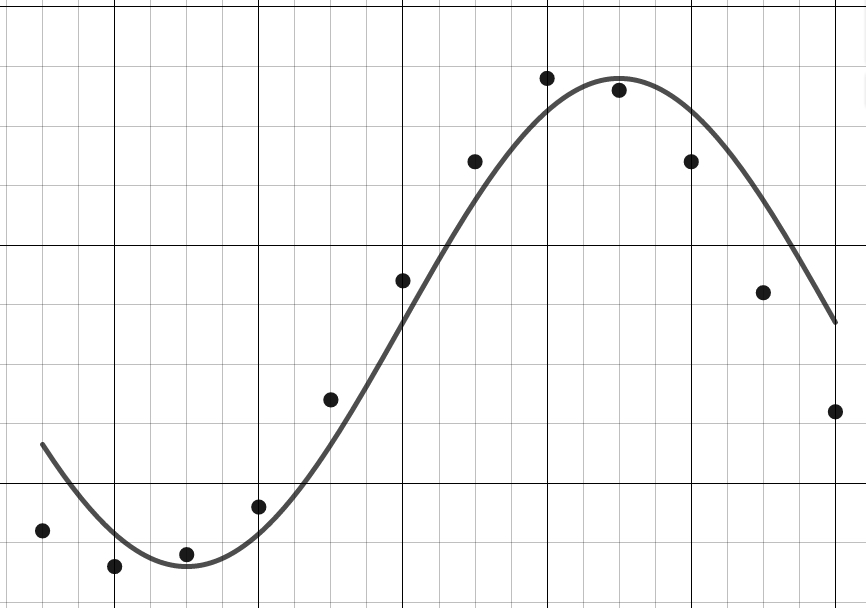
\includegraphics[height=1.5in]{./GraphsofSineandCosineGraphics/LakeErieTempReg.jpg} 

\end{center}

\item The average temperature on April $15^{\text{th}}$ is approximately $T(4.5) \approx 39.00^{\circ}$F and the average temperature on September $15^{\text{th}}$ is approximately $T(9.5) \approx 73.38^{\circ}$F.

\item  Desmos gives: $T(t) = 20.8374 \sin (-0.5251 t-0.2812) +52.3659$.  


\begin{center}

 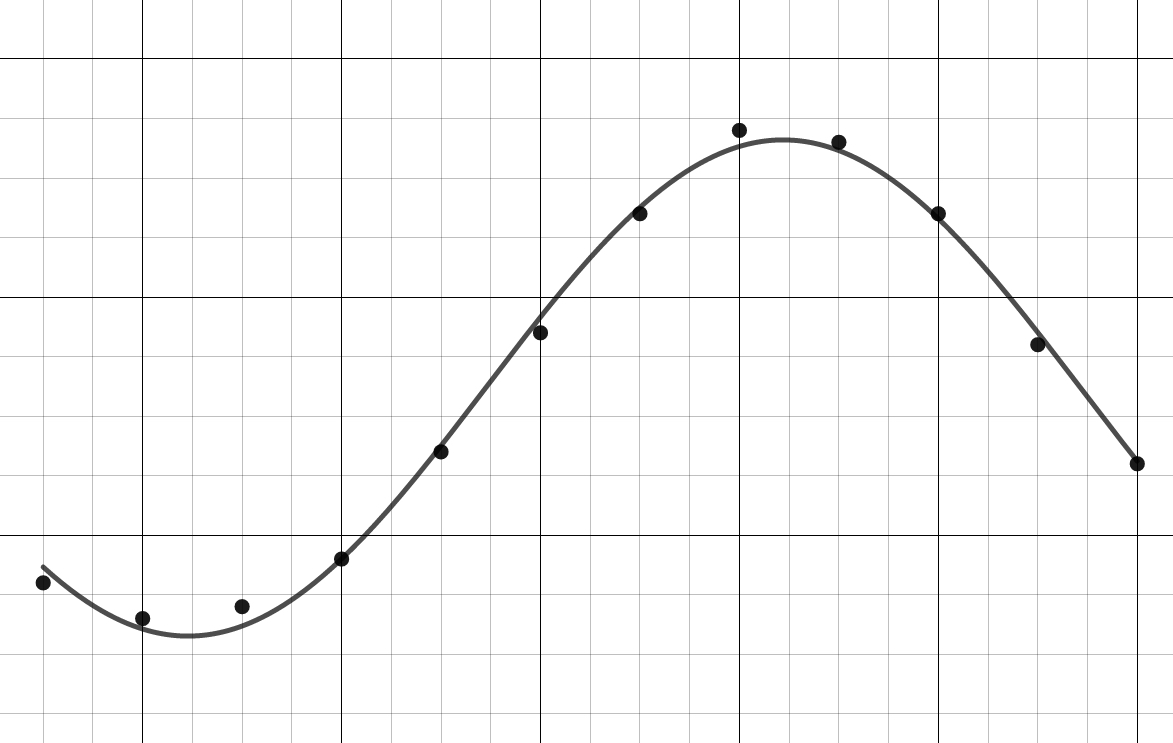
\includegraphics[height=1.5in]{./GraphsofSineandCosineGraphics/LakeErieRegDesmos.jpg} 

\end{center}

This model predicts the average temperature for April $15^{\text{th}}$ to be approximately $42.42^{\circ}$F and the average temperature on September $15^{\text{th}}$ to be approximately $70.05^{\circ}$F.  This model appears to be more accurate.

\end{enumerate}


\item  \begin{enumerate} \item  Based on the shape of the data, we either choose $A<0$ or we find the \textit{second} value of $t$ which closely approximates the `baseline' value, $F = 0.505$.  We choose the latter to obtain $F(t) = 0.475 \sin\left(\frac{\pi}{15} t - 2\pi \right) + 0.505 =  0.475 \sin\left(\frac{\pi}{15} t\right) + 0.505$ 

\enlargethispage{\baselineskip}

\item  Our function and the data set are graphed below.  It's a pretty good fit.

\begin{center}

 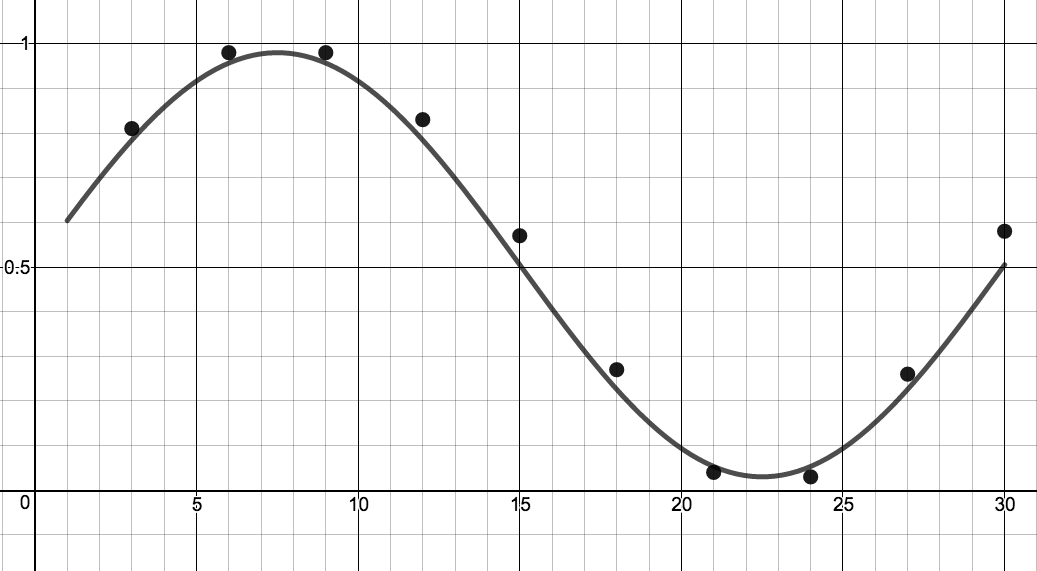
\includegraphics[height=1.5in]{./GraphsofSineandCosineGraphics/MoonIlluminationReg.jpg} 

\end{center}


\item  The fraction of the moon illuminated on June 1st, 2009 is approximately $F(1) \approx 0.60$


\item  Using desmos,\footnote{\ldots specifying $\omega = \frac{\pi}{15}$ \ldots} we get $F(t) = 0.49\sin \left(\frac{\pi }{15}t-6.29\right)+0.535$.

\begin{center}

 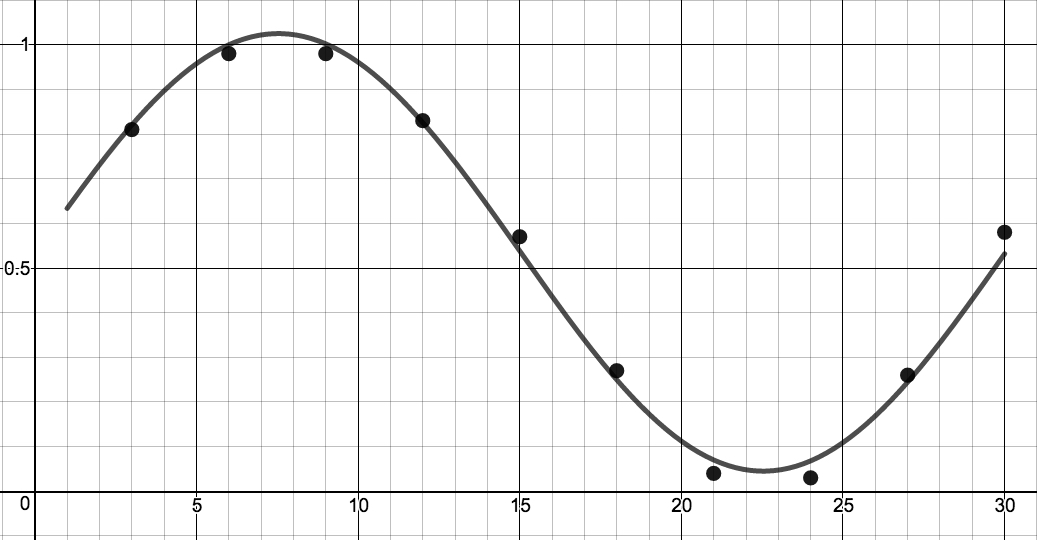
\includegraphics[height=1.5in]{./GraphsofSineandCosineGraphics/MoonIlluminatonDesmos.jpg} 

\end{center}

This model predicts that the fraction of the moon illuminated on June 1st, 2009 is approximately $0.63$.  This appears to be a better fit to the data than our first model.

\end{enumerate}


\end{enumerate}


\end{document}



\closegraphsfile